\chapter{Estabilización de la fase en OCT}
\label{chapter:estabilizacion_fase}

Uno de los problemas que se puede dar en la adquisición de datos con OCT está relacionado con la falta de sincronía en los sensores y actuadores. Este tipo de problema afecta principalmente la fase, que es importante en aplicaciones que cuantifican flujo mediante OCT. Este capítulo aborda uno de los problemas más comunes en los sistemas de OCT que emplean fuentes de barrido, y propone un método de solución que se basa en la interpretación del problema como una optimización. 

Para esto, el capítulo se divide en cinco secciones en las que se abordarán los siguientes temas: En la Sección~\ref{sec:ofdi} se retomarán los conceptos básicos detrás de OCT con fuente de barrido, en donde uno de los problemas más comunes tiene que ver con la falta de sincronía entre sus componentes, esta dificultad será tratada a fondo en la Sección~\ref{sec:estabilidad_ofdi}. Entendiendo el problema, se planteará una posible solución en la Sección~\ref{sec:propuesta_estabilidad_ofdi}, y describirá el algoritmo, sus principios y las simulaciones en la Sección~\ref{sec:algoritmo_propuesto_ofdi}. Finalmente, se discutirán los primeros resultados experimentales obtenidos con el método propuesto en la Sección~\ref{sec:resultados_experimentales_ofdi}.

\section{OCT con fuente de barrido (OFDI)}
\label{sec:ofdi}

OCT con fuente de barrido (SSOCT: \textit{swept-source optical coherence tomography}), conocido también como imagen óptica en el dominio frecuencial (OFDI: \textit{optical frequency domain imaging}), emplea una fuente de luz sintonizable para producir la interferencia entre el haz de referencia y la luz retroreflejada por la muestra, capturando el patrón de interferencia a través de las componentes espectrales de la fuente, razón por la cual no es necesario desplazar el espejo de referencia. La fuente sintonizable tiene la característica de realizar barridos espectrales con un ancho de banda instantáneo angosto a lo largo de todo el espectro, por lo que se le conoce también como fuente de barrido. El ancho de banda instantáneo corresponde al tamaño de la línea espectral que tiene la fuente mientras se realiza el barrido por las distintas componentes espectrales, de tal modo que la interferencia producida en cada instante del barrido se considera localmente coherente, pues la línea espectral instantánea en general es mucho más pequeña que el espectro total de la fuente \cite{Golubovic1997,Chinn1997,Drexler2015}.

%OCT con fuente de barrido (SSOCT: \textit{swept-source optical coherence tomography}), conocido también como imagen óptica en el dominio frecuencial (OFDI: \textit{optical frequency domain imaging}), emplea una fuente de luz sintonizable para producir la interferencia entre el haz de referencia y la luz retroreflejada por la muestra. La fuente sintonizable, tiene la característica de realizar barridos espectrales con un ancho de banda angosto o instantáneo por todo el espectro, por lo que se le conoce también como fuente de barrido. El ancho de banda instantáneo corresponde al tamaño de la línea espectral que tendrá el ancho de banda mientras se realiza el barrido por las distintas componentes espectrales. La interferencia que se produce en cada instante del barrido se considera coherente, ya que la línea el ancho espectral de la fuente en general es mucho más pequeña que el espectro, y por ende puede considerarse como coherente instantáneamente \cite{Golubovic1997,Chinn1997,Drexler2015}.

%, a este ancho de banda angosto se le denota como ancho de banda , ya que es el tamaño de la línea espectral que la fuente tendrá en algún momento determinado. 

En OFDI no es necesaria la detección con un espectrómetro a diferencia de OCT en el dominio espectral, puesto que las componentes espectrales del patrón de interferencia se encuentran codificadas sobre el barrido, en consecuencia, la señal se captura en un fotodetector como una función dependiente del tiempo sobre el periodo que tarda la fuente en realizar el recorrido por todo el espectro \cite{Drexler2015}. Es necesario entonces relacionar el instante de captura del detector con el número de onda instantáneo emitido por la fuente, la cual se espera que siga una relación lineal con respecto al tiempo \cite{Vakoc2005}. Como el número de onda $k(t)$ del patrón de interferencia registrado por el fotodetector sigue un relación lineal con el tiempo $t$, se puede describir como

\begin{equation}
k(t) = k_0 + \frac{\Delta k}{\Delta t} t,
\end{equation}

\noindent donde $k_0$ es el número de onda inicial del espectro de la fuente, $\Delta k$ es el ancho de banda del número de onda y $\Delta t$ es el periodo de barrido, inversamente proporcional a la frecuencia de la fuente. Al ser el ancho de banda espectral de la fuente finito, la profundidad de penetración máxima $z_{max}$ se encuentra limitada por las características del espectro, siendo esta

%En OFDI, la profundidad máxima de penetración $z_{max}$ se encuentra limitada por el ancho de banda espectral finito de la fuente, siendo en este caso

\begin{equation}
z_{max} = \frac{\lambda_0^2}{4\delta \lambda},
\end{equation}

\noindent donde $\lambda_0$ es la longitud de onda central ($\lambda_0 = 2\pi/k_0$), $\delta \lambda = \Delta\lambda/N_s$ es el intervalo de muestreo de la longitud de onda, $\Delta \lambda$ es la anchura a la mitad del máximo del espectro (FWHM), y $N_s$ es el número de muestras del espectro en $\Delta \lambda$. El intervalo de muestreo  $\delta \lambda$ debe ser más pequeño que el ancho de banda instantáneo de la fuente, ya que de lo contrario, la función de coherencia decaería con la profundidad, limitando el rango de penetración \cite{Drexler2015}.

OFDI es una de las técnicas de captura de datos más comunes para OCT \cite{Leitgeb2003,Choma2003} dado que posee una alta tasa de adquisición, mayor a $50kHz$ por lo que es capaz de producir más de $100$ imágenes por segundo, adicionalmente, tiene una alta sensibilidad del orden de $-120dB$, y una relación señal-ruido baja al capturar todas las profundidades de manera simultánea, viéndose menos afectado por movimientos durante la adquisición. Sin embargo, algunos de los problemas más comunes que se encuentran en OFDI están relacionados con la sincronización requerida entre el sistema de captura de datos y la fuente de barrido \cite{Vakoc2005}, éstos afectan principalmente aquellas aplicaciones en donde la fase juega un papel fundamental, y como se mencionó en la Sección~\ref{sec:plant_problemo}, hay aplicaciones de OCT que dependen altamente de variaciones en la fase, que es donde aparecen los efectos de la baja sincronía y estabilidad de la fase.

\section{Sincronización y estabilidad de fase en OFDI}
\label{sec:estabilidad_ofdi}

Debido a que la adquisición de datos en los sistemas de OCT en el dominio de Fourier se realiza de manera espectral, es necesario realizar transformadas de Fourier para relacionarlos con el dominio espacial. Como las transformadas de Fourier evalúan funciones complejas, los datos en el dominio espacial registrados con OFDI poseen valores complejos, con una amplitud y una fase asociadas. Esta característica permite que algunas aplicaciones de OCT como OCT Doppler cuantifiquen flujo a través del sensado de las variaciones de fase con respecto al tiempo entre líneas A sucesivas, lo cual es posible a través del efecto Doppler que induce el flujo sobre el haz \cite{Zhao2000}. La estabilidad de la fase se convierte entonces en una de las prioridades para aquellas aplicaciones en las que se desea obtener información confiable de cambios que solo pueden medirse a través de la fase. 

El problema de la estabilidad surge a causa de la sintonización que debe hacer la fuente de barrido en el espacio de los números de onda (espacio $k$), en donde no hay un muestreo lineal sobre el espectro, y por ende, se puede dar  una reducción en la resolución espacial del sistema \cite{Brinkmeyer1990}. Una solución para evadir este inconveniente, es que el fotodetector tenga un muestreo con intervalos de tiempo no uniformes, de manera que los datos en el detector se adquieran uniformemente con el muestreo del espacio $k$ durante todo el proceso de toma de datos. Pese a ello, si hay una falta de sincronía entre el detector y la fuente se podrían tener variaciones en la medida de la fase que degradan la sensibilidad de la técnica \cite{Drexler2015}.

La inestabilidad de fase en OFDI puede ser causada también por una variación rápida (\textit{jitter}) en la sincronización entre la fuente y el sistema de adquisición de datos. Este \jitter es un retraso de tiempo aleatorio entre la señal de disparo (\textit{trigger}) y el momento inicial de captura de datos, la incertidumbre en el tiempo de muestreo produce diferencias en el número de onda inicial para cada ciclo de la fuente \cite{Choi2013,Hong2012}. Aunque los retrasos en la señal sean pequeños, hay un impacto importante en la fase del espectro capturado y en la tasa de muestreo, manifestándose en la medida como una diferencia de fase dependiente de la profundidad (una pendiente) en conjunto con un corrimiento aleatorio de fase entre cada una de las líneas A (\textit{offset}) \cite{Liu2015}. Ahora bien, si la fuente de barrido posee componentes mecánicos tiende a tener una estabilidad de fase incluso menor, ya que comparada con una fuente sin parte mecánicas hay más causas de error \cite{Bonesi2014}. En aquellas fuentes donde elementos mecánicos realizan el barrido, el \jitter puede darse por la acumulación de momento que deriva en histéresis y desvíos indeseados, o por inestabilidades en el entorno tales como vibraciones.

Cuando un volumen de datos provenientes de OFDI se encuentre alterado a causa de la falta de sincronía entre el fotodetector y la fuente de barrido, se le denomina tomograma corrupto, ya que hay una corrupción inducida en el mapa de fase medido. Pese a que este problema se encuentra presenta en casi todas las aplicaciones de OFDI, son pocos los algoritmos existentes que permiten mejorar la estabilidad en la fase por medio de métodos numéricos o de posprocesamiento \cite{Adler2007,Vakoc2005,Hong2012,Liu2015}. Nuestro objetivo es proponer una metodología que permita ayudar con la estabilización de la fase en datos obtenidos por medio de OFDI y que presentan una corrupción en la fase por las causas descritas.


%La sincronización del muestreo entre el espacio de los números de onda (\textit{k-space}) donde se asume que la fuente trabaja en un régimen lineal, y el espacio temporal en el cual fotodetector realiza la adquisión de datos 

%\subsection{Phase-resolved optical frequency domain imaging}


\subsection{Características de los tomogramas con corrupción de fase}
\label{sec:caracteristicas_tomogramas_corruptos}

La corrupción en la fase de un tomograma se relaciona con la falta de sincronía entre la señal de disparo de la fuente y el inicio de captura de datos desde el detector. Como consecuencia de esto, hay un corrimiento aleatorio en la fase que no es evidente cuando se trabaja únicamente con la amplitud o la intensidad del tomograma. Si bien los especímenes biológicos analizados con OFDI se caracterizan por tener una fase aleatoria, las mediciones sensibles a la fase requieren de una alta estabilidad durante la captura de los datos. Para ejemplificar el efecto que tiene sobre el tomograma la presencia de corrupción en la fase se realizó una simulación de un volumen de datos con $160\times256\times256$ elementos, siendo las dimensiones respectivas $(Z,X,Y)$. La simulación se basa en el muestreo que realiza un sistema de OFDI y funciona a partir del siguiente esquema:

\begin{itemize}
\item[\textbf{Paso 1:}] Se define un volumen a escanear, tomando en consideración los tamaños físicos y las características de la fuente de barrido.
\item[\textbf{Paso 2:}] Se establece el porcentaje del volumen que estará ocupado por centros dispersores que formarán el \speckle portador de señal y el \speckle degradador de señal, por ejemplo $1\%$ del volumen ocupado por centros dispersores indica una variación en el índice de refracción bajo y por ende, una muestra relativamente homogénea; mientras que un $20\%$ quiere decir que la muestra es altamente inhomogénea.
\item[\textbf{Paso 3:}] Se asignan posiciones aleatorias a cada uno de los centros dispersores del volumen, y a continuación se añaden regiones homogéneas alrededor de algunos de los centros dispersores, formando los objetos a medir.
\item[\textbf{Paso 4:}] Se asigna de una reflectividad superior a aquellos puntos del volumen donde se encuentran los objetos, al haber múltiples centros dispersores se dará la formación de \speckle en todo el volumen, pero en aquellas regiones donde se encuentran los objetos la reflectividad será mayor, haciéndose éstos visibles.
\item[\textbf{Paso 5:}] Se realiza el muestreo del espectro en el espacio $k$, asumiendo que éste es lineal en la señal de OFDI, esto es, generar la función dependiente del tiempo que registra el detector del espacio $k$.
\item[\textbf{Paso 6:}] Para cada una de las líneas A que conforman el volumen, calcular la señal de OFDI producida por los centros dispersores y por el espectro de la fuente, a partir de la señal planteada en la Eq.~\ref{eq:i_D_1}.
\item[\textbf{Paso 7:}] Obtener la transformada de Fourier de cada línea A en el volumen para retornar la señal en el dominio espacial.
\item[\textbf{Paso 8:}] Si se desea añadir elementos de corrupción, adicionar una pendiente y un \offset en la fase de la señal en el dominio espacial, o convolucionar el espectro con una función delta que representa el corrimiento en el número de onda muestreado.
\end{itemize}


En la Fig.~\ref{fig:corruptmap} se presenta una simulación de los datos capturados por un sistema de OFDI. La intensidad del campo simulado se muestra en la Fig.~\ref{subfig:intensidad_clean}, en donde se han ubicado $12$ cilindros, como tener una corrupción en la fase no modifica la amplitud, se espera que independiente de la fase que se imponga no haya una variación en la intensidad medida. En el caso de un sistema de OCT con fuente de barrido, la fase obtenida por medio de transformadas de Fourier representa la fase aleatoria típica de los tejidos, pero con un comportamiento relativamente \textit{suave}, como se presenta en la Fig.~\ref{subfig:fase_limpia}. Sin embargo, cuando hay corrupción a causa de la falta de sincronía, como se ilustra en la Fig.~\ref{subfig:fase_corrupt}, la estructura de la fase [Fig.~\ref{subfig:fase_limpia}] se pierde, y aparecen variaciones aleatorias en la dirección $z$ (verticales) causadas por la dependencia de la fase con la profundidad (pendiente) y su inicio aleatorio (\textit{offset}) entre líneas A.

\begin{figure}[h]
	\centering
	\subfigure[Intensidad.]{\label{subfig:intensidad_clean}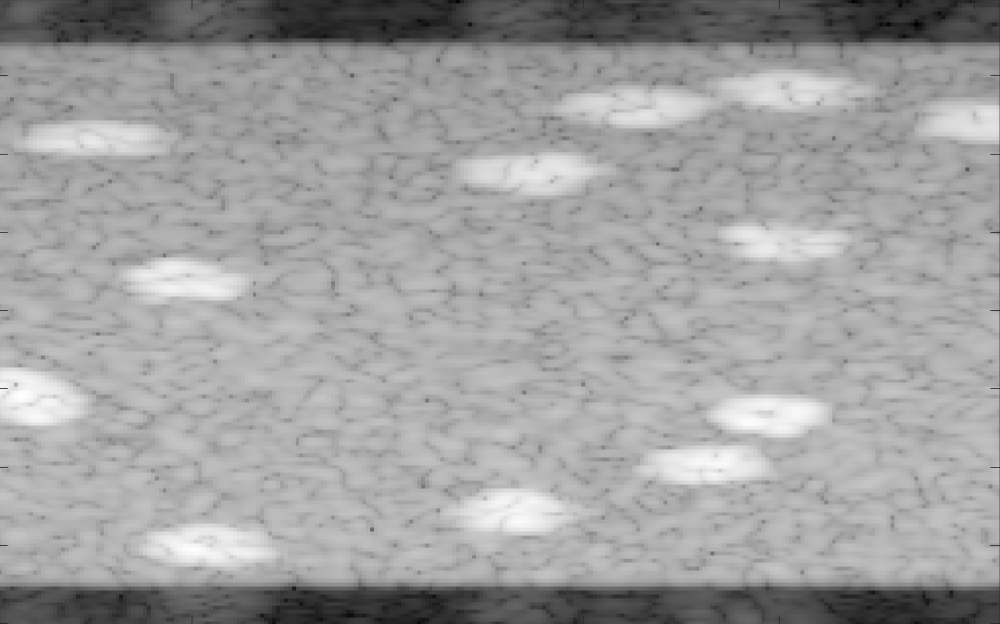
\includegraphics[width=0.3\linewidth]{img/chap4/amplitud}}
	\subfigure[Fase normal.]{\label{subfig:fase_limpia}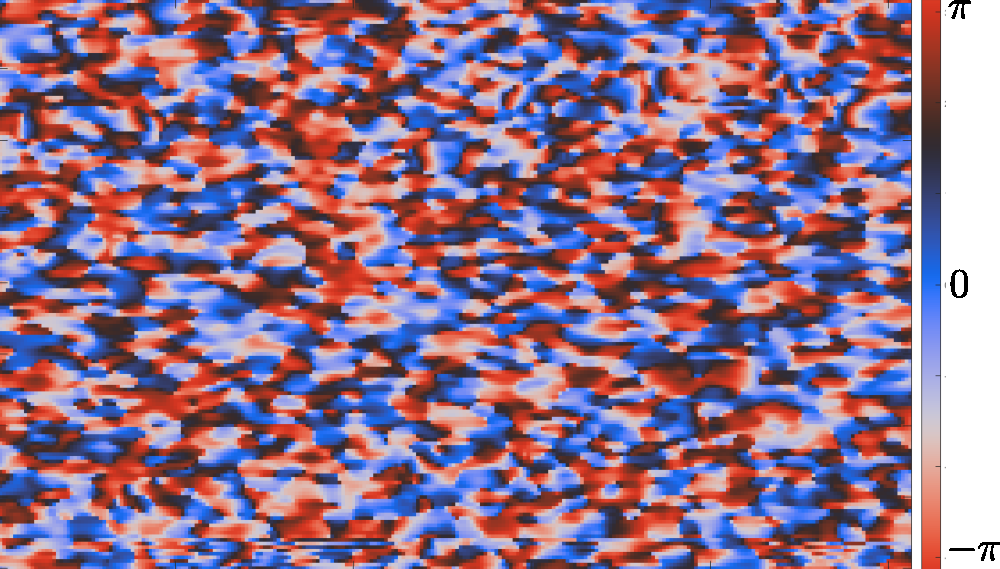
\includegraphics[width=0.33\linewidth]{img/chap4/phase_clean}}
	\subfigure[Fase corrupta.]{\label{subfig:fase_corrupt}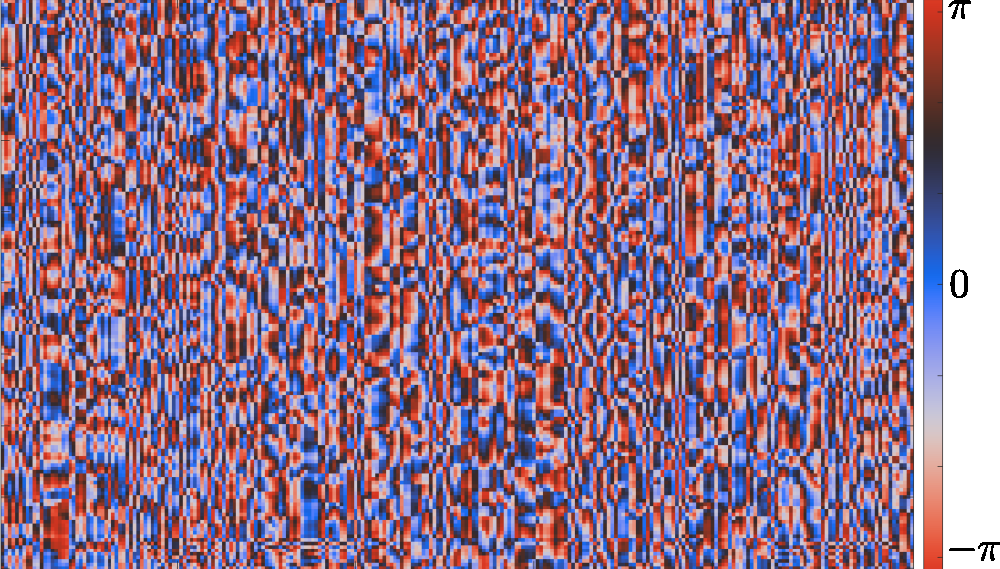
\includegraphics[width=0.33\linewidth]{img/chap4/phase_corrupt}}
	\caption[Simulación de volumen de OCT]{Comparación de una imagen simulada de OCT con fase normal y fase corrupta. (a) Intensidad del campo, (b) fase normal y (c) fase corrupta por problemas de sincronización.}
	\label{fig:corruptmap}
\end{figure}

Ahora bien, la corrupción de fase no se hace evidente en las imágenes que se muestran en el dominio espacial, ya que la intensidad no depende de la fase. No obstante, deben presentarse diferencias entre el tomograma normal y el corrupto si se toman transformadas de Fourier, puesto que éstas son sensibles ante la fase del campo complejo. En el caso del tomograma normal, su transformada de Fourier debe seguir teniendo las características del espectro capturado por OFDI antes de realizar imagen, es decir, si no hay corrupción cada línea A que conforma el volumen debe seguir teniendo las propiedades espectrales del haz con el cual se realizó la captura, esto se ilustra en la Fig.~\ref{fig:PSFComparison}. La distribución espectral del tomograma debe entonces continuar siendo una función gaussiana, similar a la que empleó para capturar los espectros que conforman el tomograma, por lo tanto, tomar la transformada de Fourier \enface del tomograma debe producir una función gaussiana reescalada similar a la empleada como iluminación. En todos estos casos se empleó una ventana \text{Hann} o \textit{Hanning} antes de tomar la transformada de Fourier para evitar la aparición de líneas verticales y horizontales por el tamaño finito de la imagen.

%Ahora bien, la corrupción de fase no se hace evidente en las imágenes que se muestran en el dominio espacial, ya que la intensidad no depende de la fase. No obstante, si se toma el campo complejo del volumen de datos y se realizan transformadas de Fourier debido a que la transformada de Fourier es sensible ante la fase, deben presentarse diferencias entre el tomograma limpio y el corrupto. En el caso del tomograma limpio, se espera que su transformada de Fourier siga teniendo las características del espectro capturado por OFDI antes de realizar imagen, es decir, si no hay corrupción, cada línea que conforma el volumen debe seguir teniendo las propiedades espectrales del haz con el cual se realizó la captura, esto se ilustra en la Fig.~\ref{fig:PSFComparison}. La aparición de la distribución espectral de la fuente se debe a que en el dominio de Fourier lo que se capturó fue la convolución entre el objeto y la función de dispersión de punto PSF para el caso de OCT (Sección~\ref{sec:int_baja_coh_fourier}), que se obtiene nuevamente si no hay elementos de corrupción. 

Si el volumen fue capturado bajo las mismas condiciones de iluminación, se espera que cada plano \enface ($XY$) tenga las características de la distribución gaussiana que sigue el haz, como lo muestra la Fig.~\ref{subfig:psf_clean} proveniente de la transformada Fourier de uno de los planos $XY$ del volumen, en donde se observa que el espectro de potencia (PS: \textit{power spectrum}, módulo cuadrado de la transformada de Fourier) del tomograma no corrupto sigue una distribución gaussiana, si se realizaran transformaciones para todos los planos $XY$ en las profundidades todos ellos seguirán esta misma distribución. Por otro lado, cuando hay elementos de corrupción de fase, la distribución que posee el haz en la transformada se pierde dado que hay una alteración aleatoria de la fase, como se puede apreciar en la Fig.~\ref{subfig:psf_corrupt}, en donde la corrupción de fase ha hecho que el PS en $XY$ aparezca como alta frecuencias distribuidas aleatoriamente. 

%Si el volumen fue capturado bajo las mismas condiciones de iluminación, se espera que cada plano \enface ($XY$) tenga las características de la distribución gaussiana que sigue el haz, como lo muestra la Fig.~\ref{subfig:psf_clean} proveniente de la transformada Fourier de uno de los planos $XY$ del volumen, si se realizaran transformaciones para todos los planos $XY$ en las profundidades todos ellos seguirán esta misma distribución. Por otro lado, cuando hay elementos de corrupción de fase la distribución que posee el haz se pierde debido a la dependencia que hay en la transformada con respecto a la fase, como se muestra en la Fig.~\ref{subfig:psf_corrupt}, en donde la corrupción ha hecho que la PSF en $XY$ aparezca como frecuencias aleatorias. 

\begin{figure}[h!]
	\centering
	\subfigure[PS para un plano $XY$.]{\label{subfig:psf_clean}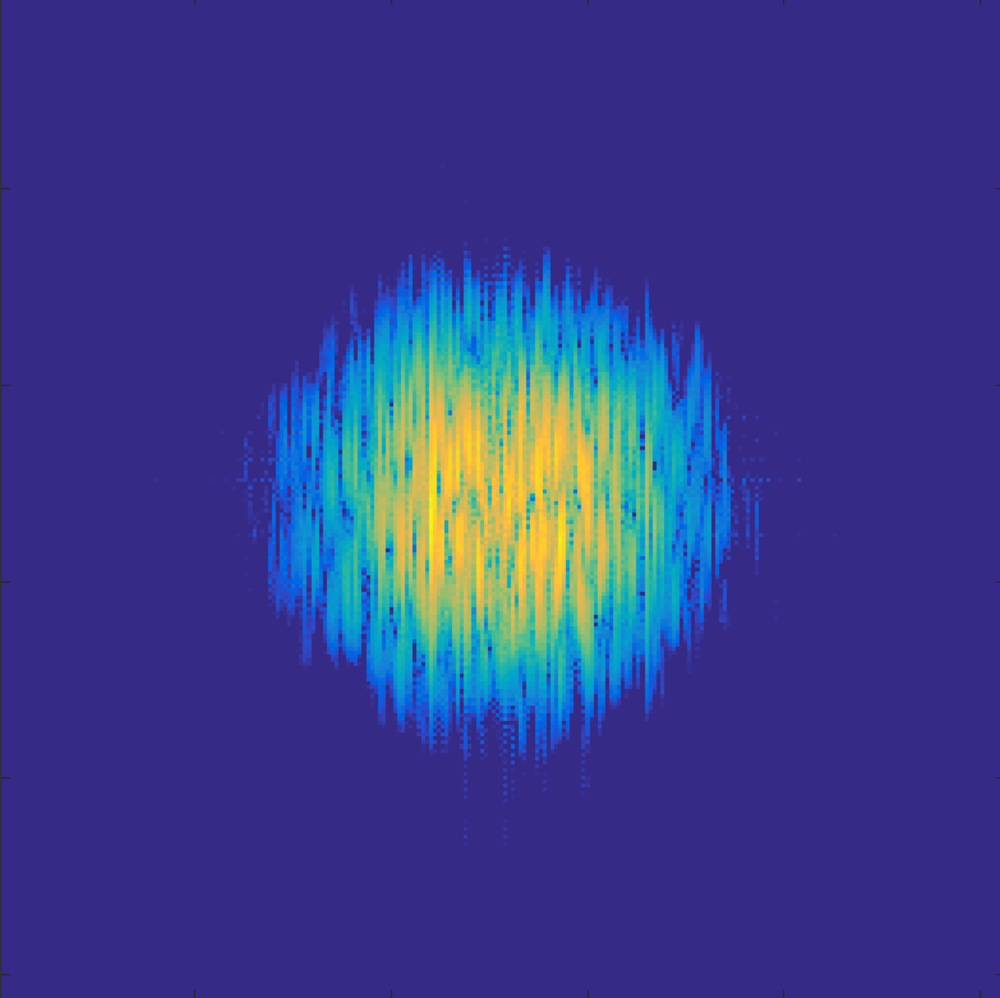
\includegraphics[width=0.19\linewidth]{img/chap4/psf_clean}}
	\subfigure[PS para un plano $XY$ corrupto.]{\label{subfig:psf_corrupt}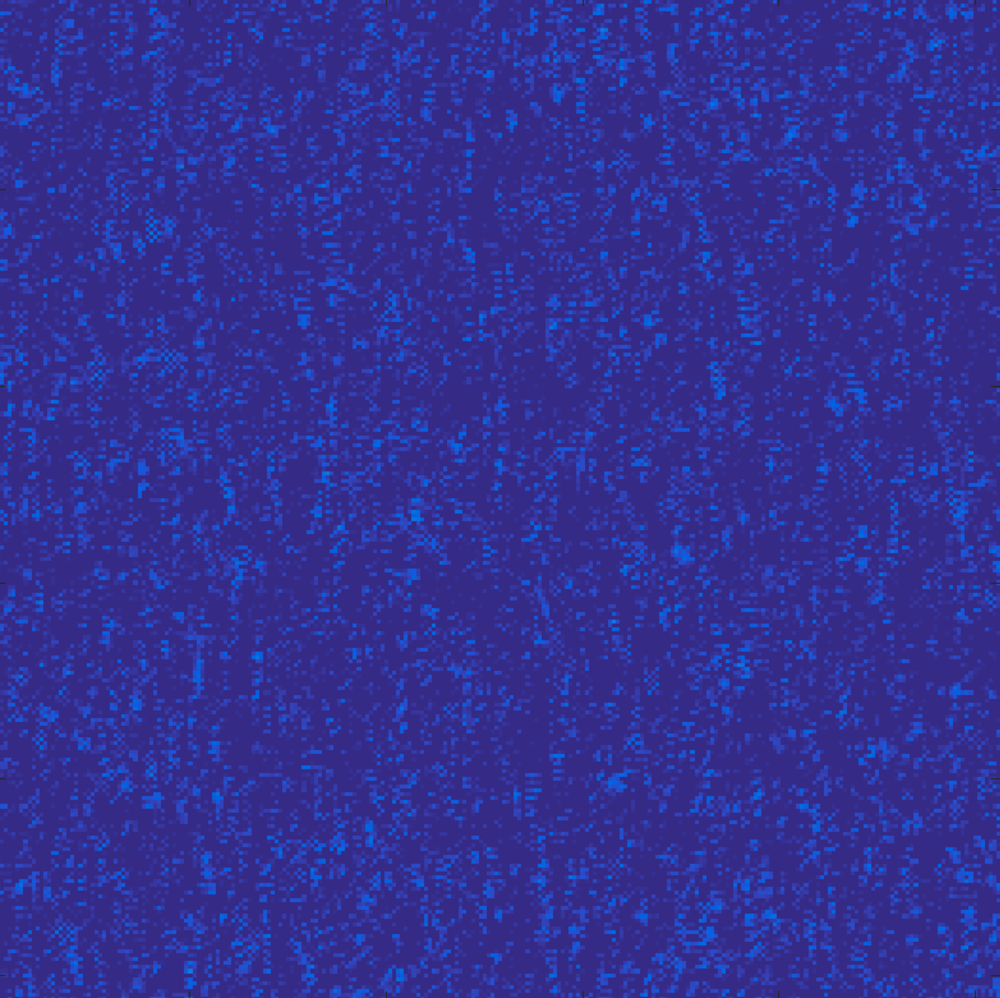
\includegraphics[width=0.19\linewidth]{img/chap4/psf_clean_pdf}}
	\subfigure[PS para un plano $XY$ con corrupción parcial.]{\label{subfig:psf_patial_corrupt}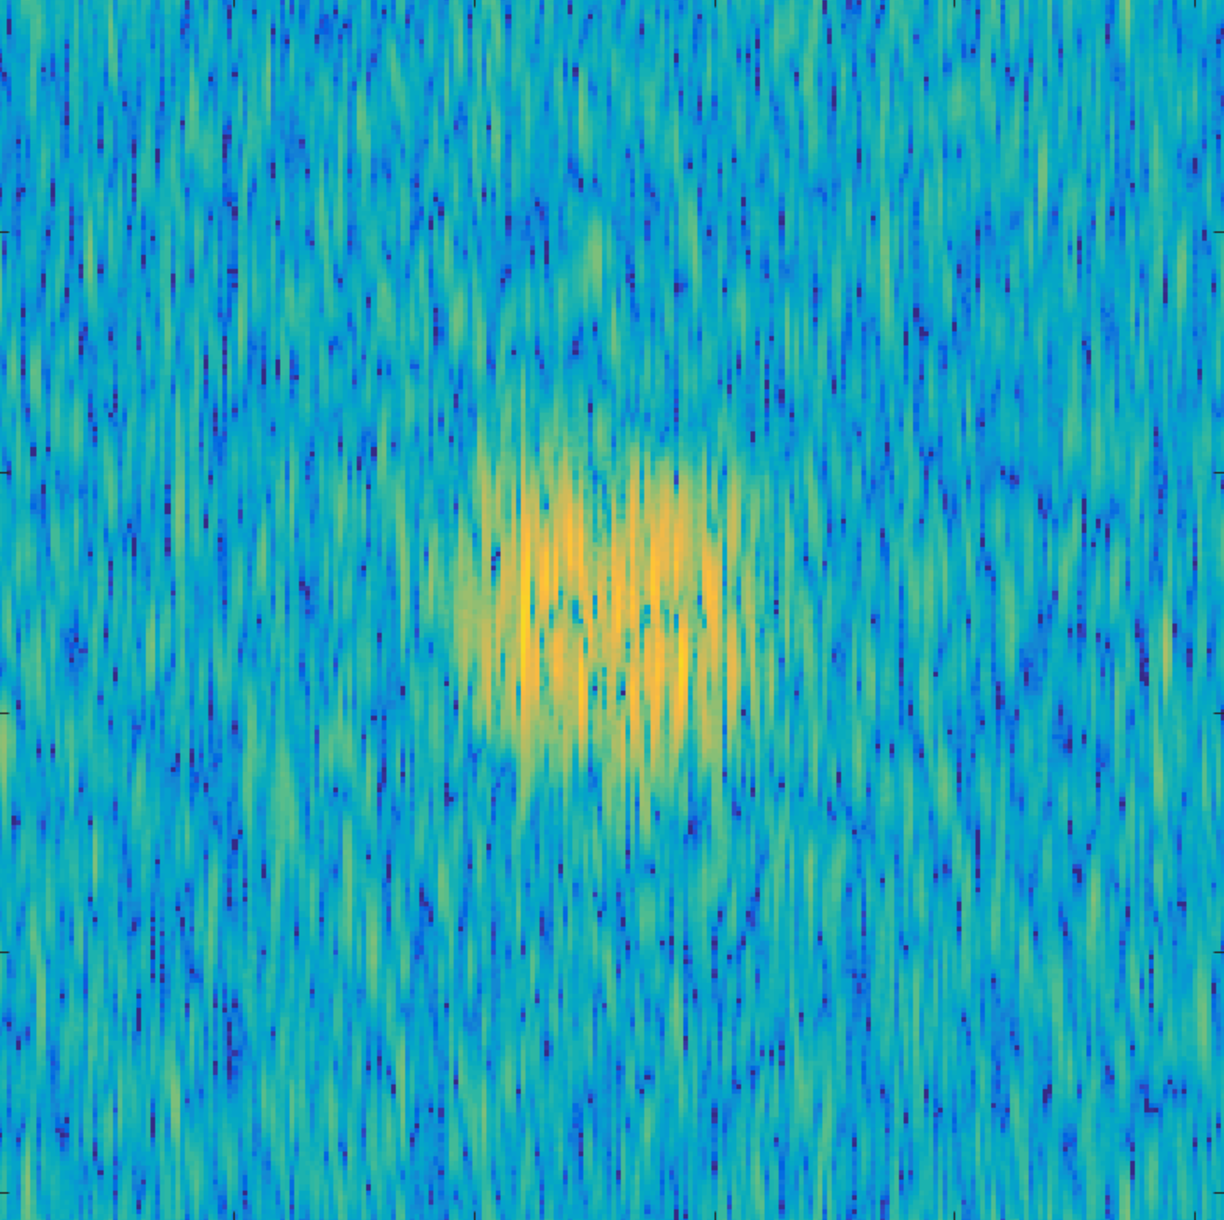
\includegraphics[width=0.19\linewidth]{img/chap4/psf_partial_corrupt}}
	\subfigure[Promedio de los PS limpias en $XY$.]{\label{subfig:psf_clean_mean}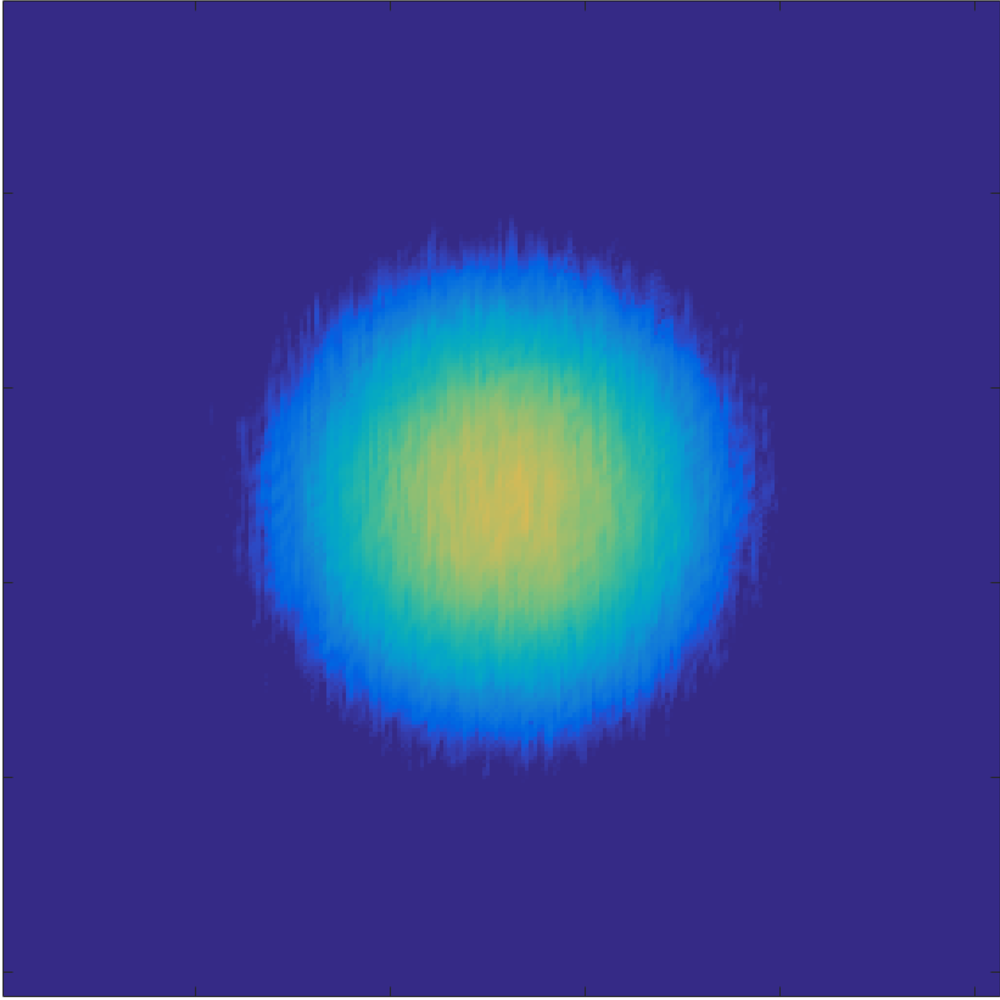
\includegraphics[width=0.19\linewidth]{img/chap4/psf_mean}}
	\subfigure[Promedio de los PS corruptas en $XY$.]{\label{subfig:psf_corrupt_mean}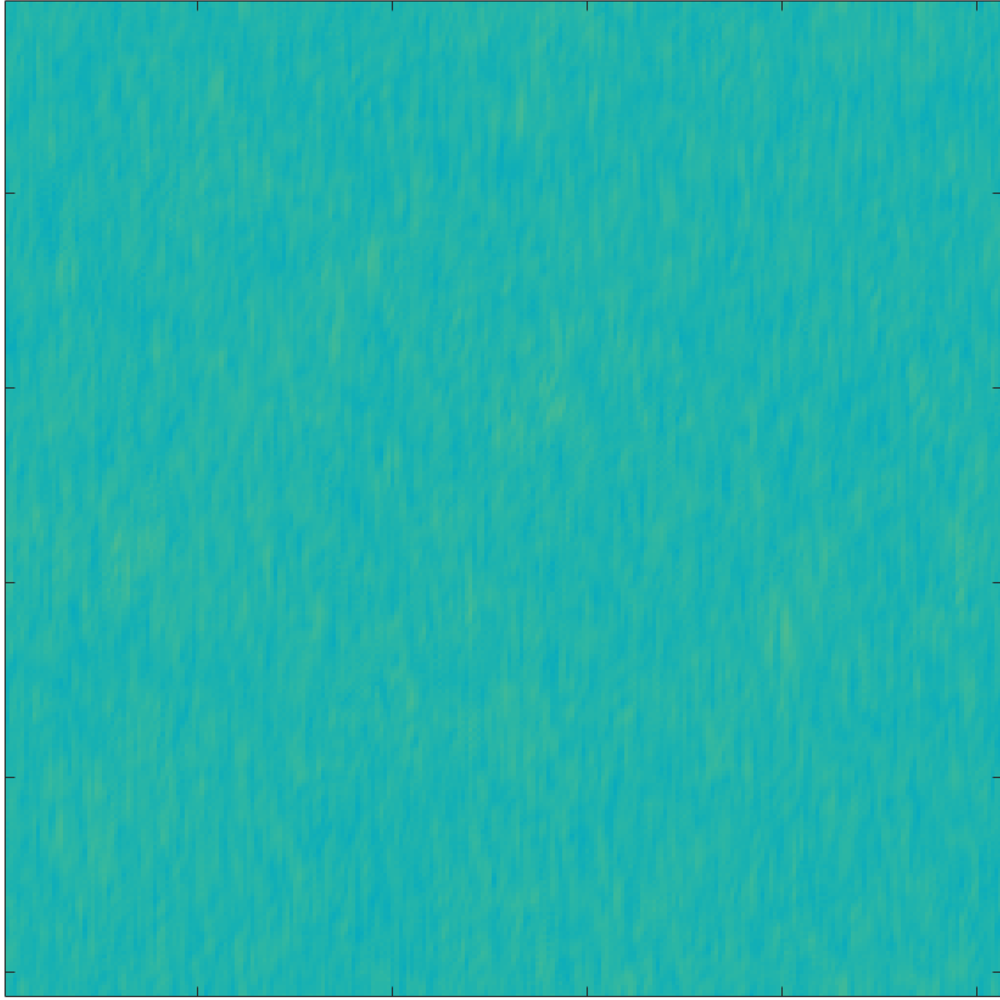
\includegraphics[width=0.19\linewidth]{img/chap4/psf_mean_corrupt}}
	\caption[Espectros de potencia con y sin corrupción]{Comparación de los PS cuando el tomograma está corrupto. (a) PS producido por un solo plano $XY$ limpio, (b) PS obtenido en un solo plano $XY$ corrupto, (c) PS generado por una corrupción parcial en la fase,(d) PS promedio del tomograma limpio, y (e) PS promedio del tomograma corrupto.}
	\label{fig:PSFComparison}
\end{figure}

%\noindent Si el error en la fase causado por el mapa de corrupción es pequeño, hay una pérdida de información al observar la PSF en $XY$, apareciendo como frecuencias altas que no corresponde con la información proveniente de la muestra y que degradan la calidad de la PSF [Fig.~\ref{subfig:psf_patial_corrupt}]. Por último, si no hay corrupción, puesto que todos los planos $XY$ del volumen poseen información sobre la PSF del sistema, si esta se promedia en todos los planos $k$ del espectro se obtiene una distribución similar a la que se empleó para capturar los patrones de interferencia, como se ejemplifica en la Fig.~\ref{subfig:psf_clean_mean}, pero cuando hay corrupción en la fase, esta relación se pierde completamente, y lo que se obtiene esencialmente es una distribución de frecuencias aleatorias al realizar el promedio, como lo muestra la Fig.~\ref{subfig:psf_corrupt_mean}.

\noindent Si el error en la fase causado por el mapa de corrupción está en el orden de los miliradianes, hay una pérdida de información al observar el PS en $XY$, apareciendo como frecuencias altas que no corresponde con la información proveniente de la muestra [Fig.~\ref{subfig:psf_patial_corrupt}]. Por último, si no hay corrupción, puesto que todos los planos $XY$ del volumen poseen información sobre el sistema, el PS promedio de todos ellos obtenido es una distribución similar que muestra un haz gaussiano definido, como se ejemplifica en la Fig.~\ref{subfig:psf_clean_mean}, pero cuando hay corrupción en la fase, esta relación se pierde completamente y lo que se obtiene es una distribución de frecuencias aleatorias al realizar el promedio, como lo presenta la Fig.~\ref{subfig:psf_corrupt_mean}.

La dependencia que hay entre el PS del sistema con respecto a la corrupción de fase debe ser posible de utilizar para caracterizar el mapa de corrupción que ha sido inducido en el volumen de datos. La idea es emplear esta información junto con la modelación que describe el mapa de corrupción en fase para recuperar el tomograma sin corrupción, o equivalentemente el mapa de corrupción, a partir de un algoritmo similar al utilizado en el enfoque de haces coherentes en medios turbios, planteando para ello un problema de optimización.

%Como lo muestra la Fig.~\ref{fig:PSFComparison} hay una alta dependencia entre la PSF en el plano $XY$ respecto al nivel de corrupción. La idea es emplear esta información junto con la modelación que describe un mapa de corrupción en fase, para recuperar el tomograma sin corrupción, o equivalentemente el mapa de corrupción a partir de un algoritmo similar al utilizado en el enfoque de haces coherentes en medios turbios, como un problema de optimización. Esta idea se describirá con más detalle en la próxima sección.

\section{Propuesta para la estabilización de la fase por posprocesamiento}
\label{sec:propuesta_estabilidad_ofdi}

Como se mencionó anteriormente, la propuesta para la estabilización de la fase consiste de dos componentes, por un lado, elementos que se han utilizado en el enfoque de haces coherentes que se propagan a través de medios turbios, y por otra parte, en el planteamiento del problema de la fase como una optimización, conociendo las características del volumen de datos normal y corrupto en OFDI. A continuación, se analizarán y describirán estos dos conceptos.

\subsection{Enfocado de haces coherentes en medios turbios}

En los medios turbios o medios altamente esparsivos y dispersivos, un haz de luz incidente es esparcido a través del medio formando un patrón de \speckle volumétrico que no posee correlación alguna en una distancia mayor a una longitud de onda. El problema se encuentra en que el patrón de \speckle producido por el medio turbio no posee un punto focal medible a la salida del sistema \cite{Vallekoop2007,Cui2011}, no obstante, si se modula el frente de onda del haz antes de ingresar al medio turbio, es posible obtener el patrón de modulación o el cambio de fase necesario para producir un enfoque del haz. Vellekoop \etal \cite{Vallekoop2007} plantearon un método para enfocar un haz que se propaga por un medio turbio, empleando un modulador espacial de luz para inducir un desfase en el haz a la entrada del sistema, y por ende, un enfoque a la salida de éste. El principio de su propuesta es que un haz enfocado produce una intensidad focal 1000 veces más grande que cuando el frente de onda no ha sido modulado. Mediante una optimización simultánea entre el haz enfocado, capturado por una cámara CCD y los niveles de gris en el modulador, los autores fueron capaces de encontrar una fase para cada uno de los 3228 puntos en los cuales se encontraba dividido el modulador, ya que cada uno de ellos producía un punto focal aproximadamente 200 veces más fuerte que el haz no enfocado. La idea de este algoritmo es obtener la fase que produce el mejor enfoque del haz y que corresponde a las variaciones globales que induce el medio turbio a través de medidas de la intensidad luego del enfoque. 

%Considerando que en los medios turbios, cada punto de la fase aporta de manera individual al enfoque del haz, ya que no hay dependencia con respecto a una vecindad del enfoque, cada uno de los elementos del modulador espacial de luz, contribuye de manera individual hasta una intensidad máxima de mejora. El proceso de optimización se basa en que el campo transmitido en la muestra $E_m$, es una combinación lineal de los campos incidentes desde los $N$ segmentos del modulador, de la siguiente manera

Considerando que en los medios turbios cada punto de la fase aporta de manera individual al enfoque del haz ya que no hay dependencia con respecto a un vecino, cada uno de los elementos del modulador espacial de luz contribuye de manera individual hasta una intensidad máxima de mejora. El proceso de optimización se basa entonces en que el campo transmitido en la muestra $E_m$, es una combinación lineal de los campos incidentes desde los $N$ segmentos del modulador, de la siguiente manera

\begin{equation}
\label{eq:e_m}
E_m = \sum_{n=1}^{N} t_{mn}A_ne^{i\phi_n},
\end{equation}

\noindent donde $A_n$ y $\phi_n$ son la amplitud y la fase de luz del segmento $n$. El esparcimiento que experimenta la luz al pasar por la muestra y propagarse por el sistema óptico se describe a través de los elementos $t_{mn}$. Si los términos de $E_m$ en la Eq.~\ref{eq:e_m} se encuentran en fase, entonces, la magnitud del campo transmitido será máxima. La fase de cada segmento, se determina mediante una variación cíclica entre $0$ y $2\pi$ en un proceso iterativo hasta que se obtiene un valor máximo para $E_m$. %En el caso de un medio turbio, las propiedades estadísticas de todos los elementos $t_{mn}$ son independientes. 

La idea de la implementación de este algoritmo al caso de corrupción en fase por inestabilidad en OCT, surge entonces como un análogo al enfoque en medios turbios planteado por Vallekoop \etal \cite{Vallekoop2007}. La propuesta es aplicar los conceptos del enfoque, pero comprendiendo que en el caso de OCT deben haber algunas variaciones en el planteamiento del algoritmo, ya que en lugar de modelar la fase que produce el mejor enfoque, buscaremos aquella pendiente y aquel \offset que aproximan el PS del tomograma corrupto a aquel producido por un sistema sin corrupción, entendiendo este problema como el \textit{enfoque} del tomograma corrupto.%, esta idea se expondrá a fondo en la siguiente sección.

\section{Algoritmo propuesto}
\label{sec:algoritmo_propuesto_ofdi}

%Como se mostró en la Sección~\ref{sec:caracteristicas_tomogramas_corruptos}, si la corrupción en la fase del tomograma es parcial [Fig.~\ref{subfig:psf_patial_corrupt}] la PSF producida por cada plano $XY$, y por consiguiente, la PSF promedio tienden a ser como aquella PSF no corrupta [Fig.~\ref{subfig:psf_clean_mean}]. Sabemos también que el \offset y la pendiente en la fase de cada una de las líneas A del volumen son diferentes, pero es la misma para todos los puntos $z$ de la línea A. En el caso de enfoque en medios turbios, si se encuentra la fase global que introduce el medio en cada uno de los puntos del modulador, se mejora altamente la intensidad de enfoque; en el caso de OCT, cuando el tomograma está corrupto, la PSF promedio que produce pierde completamente la forma gaussiana, sin embargo, si es posible encontrar una combinación pendiente-\offset y aplicar su inversa al tomograma corrupto, debe ser posible recuperar la PSF del sistema que no tiene corrupción. Por lo tanto, partiendo de conocer que cada línea A posee un \offset y una pendiente, y que su tranformada de Fourier no produce la PSF del sistema, tendría que ser factible encontrar esa misma combinación para cada línea A que corrige la corrupción en el tomograma. Bajo este principio e inspirados en la propuesta de Vallekoop \etal \cite{Vallekoop2007}, se propone un algoritmo que evalúa el \offset y la pendiente en cada una de las líneas A que conforman el tomograma, a fin de que por la PSF promedio se recupere el mapa de corrupción que producen una PSF no corrupta.% Para este fin, a continuación se discute el planteamiento del problema.

Como se presentó en la Sección~\ref{sec:caracteristicas_tomogramas_corruptos}, si la corrupción en la fase del tomograma es parcial [Fig.~\ref{subfig:psf_patial_corrupt}] el PS producido por cada plano $XY$, y por consiguiente, el PS promedio tienden a ser como aquel PS cuando el tomograma no está corrupto [Fig.~\ref{subfig:psf_clean_mean}]. Sabemos también que el \offset y la pendiente en la fase de cada una de las líneas A del volumen corrupto son diferentes, pero son las misma para todos los puntos $z$ de la línea A. En el caso de enfoque en medios turbios, si se encuentra la fase global que introduce el medio en cada uno de los puntos del modulador, se mejora altamente la intensidad de enfoque; en el caso de OCT, cuando el tomograma está corrupto, el PS promedio que produce pierde completamente la forma gaussiana, sin embargo, si es posible encontrar una combinación pendiente-\offset y aplicar su inversa al tomograma corrupto, debe ser viable recuperar el PS del tomograma que no tiene corrupción. Por lo tanto, partiendo de conocer que las líneas A con un \offset y una pendiente producen un PS con altas frecuencias aleatorias, tendría que ser factible encontrar la combinación correspondiente para cada línea A que produce el PS correcto. Bajo este principio e inspirados en la propuesta de Vallekoop \etal \cite{Vallekoop2007}, se propone un algoritmo que evalúa el \offset y la pendiente en cada una de las líneas A que conforman el tomograma corrupto, a fin de que a través del PS promedio se recupere el mapa de corrupción.% Para este fin, a continuación se discute el planteamiento del problema.

Durante la adquisición de datos de un tomograma a través de OFDI, se realiza la medición de un conjunto de $N$ espectros $S_n(k)$ que se encuentran corruptos por la falta de sincronización entre el \textit{trigger} de la fuente y el sistema de adquisición de datos. El índice $n$ denota la línea A correspondiente capturada, por lo tanto, $S_1(k)$ será el primer espectro que es la referencia global para los espectros siguientes $S_2(k), S_3(k), \ldots, S_N(k)$, además, cada línea A tiene un muestreo de $M$ puntos. En este orden de ideas, se puede relacionar a $M$ y $N$ con la cantidad de puntos o muestras en la dirección $z$ y en las direcciones laterales $xy$ respectivamente. Para obtener el tomograma en el dominio espacial, es necesario tomar la transformada de Fourier $F_n(z)$ de cada uno de los espectros que conforman el volumen, de manera que $F_n(z)$ se relaciona con $S_n(k)$ por una transformada de Fourier $\mathscr{F}_{z} \big\{S_n(k)\big\} = F_n(z)$, el índice $z$ de la transformada indica que esta se realiza sobre la dirección $z$. Debido a la influencia de la sincronía en la captura de los espectros, el tomograma sin corrupción $F^{\ast}_n(z)$ y su espectro $S^{\ast}_n(k)$ son completamente desconocidos, pero el tomograma sin corrupción se relaciona con el corrupto por la presencia de un \offset $\varphi_n$ y una pendiente $\xi_n$ (que depende de la profundidad) aleatoria para cada línea A, entonces, se puede describir el tomograma corrupto a partir del no corrupto como


%Sea $S_n(k)$ el conjunto de $N$ espectros capturado por un sistema de OFDI que se encuentra influenciado por falta de sincronía entre la fuente de barrido y el detector, de forma que $S_1(k)$ es el primer espectro capturado que es la referencia global para los siguientes espectros $S_2(k), S_3(k),\ldots,S_N(k)$. Sea $F_n(z)$ la transformada de Fourier del espectro $S_n(k)$, y por ende el tomograma en el dominio espacial formado por $N$ líneas A. Debido a la influencia de la sincronía en la captura de los espectros, el tomograma sin corrupción $F^{\ast}_n(z)$ y su espectro $S^{\ast}_n(k)$ son completamente desconocidos, pero el tomograma sin corrupción se relaciona con el corrupto por la presencia de un \offset $\varphi_n$ y una pendiente $\xi_n$ aleatoria para cada línea A, de forma que el modelo que sigue el tomograma corrupto es

\begin{equation}
\label{eq:f_n}
F_n(z) = F_n^{\ast}(z)e^{i2\pi z\frac{\xi_n}{M}}e^{i2\pi \varphi_n},
%F_n(z) = F_n^{\ast}(z)e^{i2\pi \left[\varphi_n + \frac{\xi_n}{M}z\right]},
\end{equation}

\noindent donde $i$ es la unidad imaginaria. Como la pendiente que se introduce puede tener un valor cualquiera su rango será $0\leq\xi_n<\infty$, mientras que el \offset es una característica cíclica que indica el momento de inicio de adquisición, por ende se define en el intervalo $0\leq\varphi_n<1$. En la Eq.~\ref{eq:f_n} el aporte de la pendiente $\xi_n$ está relacionado con la dependencia de la fase con la profundidad, mientras que el \offset $\phi_n$ es un valor constante que produce un desfase de la línea A. Nótese que la amplitud de los tomogramas relacionados en la Eq.~\ref{eq:f_n} no se ve influenciada por la presencia del \offset o la pendiente, ya que estos valores son complejos, la amplitud es entonces la misma para el caso con y sin corrupción. Ahora bien, el problema se encuentra en determinar $\xi_n$ y $\phi_n$ para cada una de las líneas A del tomograma, exceptuando la primera $n=1$ que es la referencia global.

En vista de que no conocemos los datos sin corrupción, realizamos una estimación $\hat{F}_n(z)$ que representa a $F^{\ast}_n(z)$ $\left[F^{\ast}_n(z) \triangleq \hat{F}_n(z)\right]$ a partir del tomograma corrupto $F_n(z)$ por medio de la siguiente relación,

%\begin{equation}
%F^{\ast}(z) \triangleq \hat{F}_n(z)
%\end{equation}


\begin{equation}
\label{eq:f_est}
\hat{F}_n(z) = t_n(z) F_n(z),
\end{equation}

\noindent donde el parámetro $t_n$ corresponde al inverso de la corrupción que posee la línea A, así

\begin{equation}
t_n(z) = e^{-i2\pi z \frac{\hat{\xi}_n}{M}}e^{-i2\pi \hat{\varphi}_n}.
\end{equation}

\noindent Nuestro objetivo es calcular la pendiente $\hat{\xi}_n$ y el \offset $\hat{\varphi}_n$ a partir de los datos del tomograma corrupto, para esto se utilizará la información disponible al tomar las transformadas de Fourier ($\mathscr{F}_{xy}$) sobre los planos $XY$ que como se analizó en la Sección~ \ref{sec:caracteristicas_tomogramas_corruptos}, producen que el PS sea una función gaussiana o una distribución aleatoria. El tomograma no corrupto $F^{\ast}_n(z)$ produce un PS con perfil gaussiano $\zeta^{\ast}_m(k)$ al tomar su transformada de Fourier sobre el plano $XY$ en todas las profundidades, esto es

\begin{equation}
\zeta^{\ast}_m(k) = \bigg\lvert \mathscr{F}_{xy} \big\{F^{\ast}_n(z)\big\}\bigg\rvert^2,
\end{equation}

\noindent y por tanto el promedio $\zeta^{\ast}(k)$ de todas los PS en $XY$ en las $M$ muestras, se define como

\begin{equation}
\zeta^{\ast}(k) = \frac{1}{M}\sum_{m=1}^{M} \zeta^{\ast}_m(k).
\end{equation}

\noindent Se espera que en un tomograma no corrupto, el PS promedio sea como el que se planteó en la Fig.~\ref{subfig:psf_clean_mean} y que por tanto, si los parámetros $\hat{\xi}_n$ y $\hat{\varphi}_n$ son la corrupción de fase, este sea el PS que se obtenga. Sin embargo, en datos experimentales no se conoce $F^{\ast}_n(z)$ ni $\zeta^{\ast}(k)$, pero se sabe que el PS para el tomograma no corrupto puede calcularse a partir de las características físicas del haz como una distribución gaussiana, por lo tanto, el cálculo de $\zeta^{\ast}(k)$ en base a las propiedades del haz se define como $\zeta^{\dagger}(k) \triangleq \zeta^{\ast}(k)$.

%\begin{equation}
%\zeta^{\dagger}(k) \triangleq \zeta^{\ast}(k).
%\end{equation}

Ahora bien, si se toma la transformada de Fourier para cada plano $XY$ en donde se ha estimado $\hat{\xi}_n$ y $\hat{\varphi}_n$ es posible obtener el PS promedio estimado $\hat{\zeta}(k)$ desde cada una de las muestras del PS en el caso corrupto $\hat{\zeta}_m(k)$ como

\begin{align}
\label{eq:zeta_m_y_prom}
\hat{\zeta}_m(k) = &\bigg\lvert \mathscr{F}_{xy} \left\{\hat{F}(z)\right\}\bigg\rvert^2 \notag\\
\hat{\zeta}(k) = &\frac{1}{M}\sum_{m=1}^{M} \hat{\zeta}_m(k).
\end{align}

\noindent Si los parámetros $\hat{\xi}_n$ y $\hat{\varphi}_n$ son la pendiente y el \offset que corrompen el volumen, entonces el PS promedio estimado $\hat{\zeta}(k)$ debe ser igual a aquel generado con los parámetros del haz $\zeta^{\dagger}(k)$, por ende, este problema puede plantearse como una optimización a través de un funcional o función de mérito $L(\hat{\xi}_n,\hat{\varphi}_n)$ que relaciona los PS partir del \offset y la pendiente estimados, de la siguiente manera

\begin{equation}
\label{eq:L}
\min \left[L(\hat{\xi}_n,\hat{\varphi}_n)\right] = {\bigg\lvert \zeta^{\dagger}(k) - \hat{\zeta}(k)\bigg\rvert^2}.
\end{equation}

La función de mérito de la Eq.~\ref{eq:L} podría resolverse por métodos de optimización, tales como el \textit{nelder-mead}, sin embargo, debido a que hay dos variables independientes por cada línea A, el tiempo de procesamiento, el consumo de memoria y la cantidad de iteraciones del algoritmo harían el cálculo tedioso. En lugar de esto, la propuesta es resolver este problema con un esquema similar al planteado por Vellekoop \cite{Vallekoop2007}, en donde la optimización se realiza secuencialmente en cada una de las líneas A, calculando los cambios en la función de mérito cuando se realiza un cambio del \offset estimado $\hat{\varphi}_n$ y de la pendiente estimada $\hat{\xi}_n$. Para esto se evalúa un intervalo de búsqueda de $j$ valores diferentes en cada iteración, por ejemplo, en la primera iteración, pueden evaluarse cuatro posibles valores para la pendiente y el \offset en un rango de $2\pi$, es decir que en este caso $j$ tomaría valores $\{-\pi, \pi/2, 0, \pi/2\}$. Dependiendo de la precisión que se quiera en el algoritmo, se evaluarán pasos más finos del intervalo y se incrementarán la cantidad de iteraciones que éste realiza, entendiendo que la iteración se da al calcular todas las líneas A del volumen e incrementar las $j$ divisiones del intervalo de búsqueda.

La hipótesis es que así como la intensidad de enfoque se incrementa altamente cuando se calcula correctamente la fase para enforcar el medio turbio, si el \offset y la pendiente están cerca de los valores reales al tomar alguno de los factores de $j$, debe haber un incremento significativo en la aproximación que se hace del PS al tomar la transformada de Fourier sobre el plano $XY$ y realizar el promedio, lo que produce variaciones significativas en la función de mérito objetivo. Cuando $L(\hat{\xi}_n,\hat{\varphi}_n)$ tiene un valor de cero, es que los PS calculados son iguales y por ende, se ha calculado la pendiente $\xi_n$ y el \offset $\varphi_n$ que cada línea A posee ya que solo éstas determinan su diferencia. Como se está calculando un rango discreto de valores, el algoritmo tendrá un error mínimo asociado a la imposibilidad de evaluar los infinitos números que hay en un intervalo. Puesto que el algoritmo debe evaluar un conjunto de valores para cada línea A, se sugiere que se realice el proceso iterativo comenzando con la evaluación de pocos puntos $j$ y se escoja como \offset estimado $\hat{\varphi}_n$ y pendiente estimada $\hat{\xi}_n$ el que produzca la mayor reducción en la función de mérito, así se garantiza que no se tomarán valores que se alejen de la solución. La evaluación de la pendiente y el \offset debe realizarse de manera separada calculando secuencialmente éstas en el volumen de datos y su PS, o a través de la generación de una maya que describa las variaciones en la función de mérito de acuerdo al intervalo evaluado para un caso bidimensional.


\subsection{Metodología del algoritmo de optimización de fase}

Para evaluar el algoritmo propuesto se requiere como entrada el tomograma corrupto $F_n(z)$, la estimación del PS no corrupto $\zeta^\dagger(k)$, el número $N$ de líneas A, el número de muestras $M$ de $z$ y los valores del intervalo que se le asignarán a $\hat{\xi}_n$ y $\hat{\varphi}_n$ en cada iteración. A continuación, hay que realizar el cálculo de la función de mérito inicial, tomando la transformada de Fourier $\mathscr{F}_{xy}$ de $F_n(z)$ y obteniendo el valor promedio del PS $\hat{\zeta}(k)$, esta primera aproximación $\min[L(\hat{\xi}_n,\hat{\varphi}_n)]$ indica el valor que la estimación de la pendiente y el \offset deben mejorar. Luego, se debe evaluar la pendiente y el \offset para cada uno de los valores del intervalo elegido, si alguno de éstos disminuye la función objetivo es porque está más cerca de los parámetros de corrupción, entonces se debe fijar la pendiente estimada $\hat{\xi}_n$ y el \offset estimado $\hat{\varphi}_n$ al nuevo valor en evaluación $\hat{\xi}^j_n$ y $\hat{\varphi}^j_n$. Por el contrario, si el valor evaluado no produce una disminución en la función de mérito, entonces se debe dejar el valor actual que tiene la pendiente y el \offset estimados, y seguir con los demás valores del intervalo. La función de mérito disminuirá gradualmente cuando en cada uno de los puntos del intervalo $j$ se evalúen, y de éstos se escoja el que produce la menor función de mérito. Una semilla para este algoritmo puede ser impuesta en los valores iniciales de $\hat{\xi}_n$ y $\hat{\varphi}_n$.

El proceso de cálculo debe repetirse para cada una de las $N$ líneas A, de forma que al terminar la iteración en curso se habrán calculado nuevos valores estimados para $\hat{\varphi}_n$ y $\hat{\xi}_n$. Al obtener entonces la función de mérito inicial para la siguiente iteración con nuevos valores en el intervalo $j$, la disminución que ha tenido la función, hará que el algoritmo únicamente varíe $\hat{\varphi}_n$ y $\hat{\xi}_n$ si los valores en la iteración actual son mejores que la anterior. La aproximación gradual entre los PS estimados hace que se almacenen los valores que mejor representan la pendiente y el \offset del tomograma, hasta que se alcanza una convergencia por la cantidad de iteraciones que realiza el algoritmo. Los últimos valores almacenados para $\hat{\varphi}_n$ y $\hat{\xi}_n$ corresponderán con aquellos que mejor representan el mapa de corrupción del tomograma y se espera que así se pueda corregir la fase. Los pasos que sigue el algoritmo de optimización de fase se describen en el Algoritmo~\ref{alg:optalgo}.

\begin{algorithm}
	\begin{tabularx}{0.8\textwidth}{l}
		
		%	\hline
		\textbf{Entrada:} tomograma corrupto $F_n(z)$, estimación del PS $\zeta^\dagger(k)$,\\
		número de iteraciones y valores a evaluar $j$, semilla $\hat{\xi}_n$ y $\hat{\varphi}_n$.\\
		\hline
		\hspace*{0.6cm}\textbf{Inicio:} Evaluar cada valor de $j$ en todas las iteraciones.\\
		\hspace*{0.6cm}\textbf{Para} $valores \hspace*{0.2cm} j \hspace*{0.2cm} hasta \hspace*{0.2cm} completar \hspace*{0.2cm} iteraciones$\\
		\hspace*{0.9cm} \textbf{Fijar} $valores \hspace*{0.2cm} de \hspace*{0.2cm} j$ \textbf{hacer}\\
		\hspace*{0.9cm} Calcular $\min[L(\hat{\xi}_n,\hat{\varphi}_n)]$ con semilla.\\
		\hspace*{0.9cm} \textbf{Para} cada línea A $n\in N$\\
		\hspace*{1.2cm} Evaluar valores de $\hat{\xi}^j_n$ y $\hat{\varphi}^j_n$ en $j$.\\
		\hspace*{1.2cm} \textbf{Para} todo valor en $j$ \textbf{hacer}\\
		\hspace*{1.5cm} Calcular $\hat{F}_n(z)$ con Eq.~\ref{eq:f_est} \textbf{luego}\\ 
		\hspace*{1.5cm} Calcular $\hat{\zeta}(k)$ con Eq.~\ref{eq:zeta_m_y_prom} \textbf{luego}\\
		\hspace*{1.5cm} Evaluar $L(\hat{\xi}^j_n,\hat{\varphi}^j_n)$\\
		\hspace*{1.5cm} \textbf{Si} $L(\hat{\xi}^j_n,\hat{\varphi}^j_n) < \min[L(\hat{\xi}_n,\hat{\varphi}_n)]$ \textbf{entonces}\\
		\hspace*{1.8cm} \textbf{Fijar} Nuevos valores estimados\\
		\hspace*{1.8cm} $\min(L(\hat{\xi}_n,\hspace*{0.2cm} \hat{\varphi}_n))=L(\hat{\xi}^j_n,\hspace*{0.2cm}\hat{\varphi}^j_n),\hspace*{0.2cm} \hat{\varphi}_n=\hat{\varphi}^j_n,\hspace*{0.2cm} \hat{\xi}_n=\hat{\xi}^j_n$\\
		\hspace*{1.5cm} \textbf{FinSi}\\
		\hspace*{1.2cm} \textbf{FinPara}\\
		\hspace*{0.9cm} \textbf{FinPara}\\
		\hspace*{0.9cm} Pasar a siguientes valores de $j$.\\
		\hspace*{0.6cm}\textbf{FinPara}\\
		\hspace*{0.6cm}\textbf{Salida:} Retornar $\hat{\xi}_n, \hat{\varphi}_n$.\\
		%	\hline	
		
	\end{tabularx}
	\caption{Implementación del algoritmo optimización de fase.}
	\label{alg:optalgo}
\end{algorithm}

\subsection{Simulaciones}

Para probar el algoritmo propuesto, se emplearon los datos de la simulación presentada en la Sección~\ref{sec:caracteristicas_tomogramas_corruptos} y se le agregó al tomograma mapas de corrupción con diferentes rangos aleatorios del \offset y la pendiente para evaluar los valores máximos que el algoritmo puede recuperar. Para la evaluación se emplearon $N = 32\times32$ líneas A con $M = 160$ muestras en profundidad y se tomó como PS promedio objetivo $\zeta^{\dagger}(k)$ el calculado con los datos antes de aplicar la corrupción, adicionalmente, el rango de \textit{offsets} y pendientes estimados se varío gradualmente entre iteraciones en $4, 8, 16, 32, 64, 128$ y $256$ muestras de un intervalo de $2\pi$.

La evaluación de escalas bajas para los valores aleatorios del mapa de corrupción, entre $0$ y $\pi$, mostraron resultados satisfactorios en el tomograma con fase corregida. Para discutir esto, en la Fig.~\ref{fig:ps_pi} se presenta la evolución del PS con respecto a las iteraciones del algoritmo y en la Fig.~\ref{fig:phase_pi} se comparan las fases obtenidas para un mapa de corrupción con valores de \offset y pendiente distribuidos en un rango de $\pi$. En el caso de los espectros de potencia, se observa en la Fig.~\ref{subfig:PI_ps_clean} que cuando no hay corrupción de fase sigue una distribución gaussiana con pocas componentes de altas frecuencias, mientras que cuando se aplica la corrupción, se ven más componentes de frecuencias altas pero se observan características gaussianas [Fig.~\ref{subfig:PI_ps_init}], en este caso, la función de mérito inicial correspondía a $745$, siendo esta la máxima diferencia. 

Con las evaluaciones de la pendiente y el \textit{offset} la distribución aleatoria de la corrupción lentamente se acerca a la del tomograma no corrupto, como lo ilustran las Figs.~\ref{subfig:PI_ps_5iter} y \ref{subfig:PI_ps_15iter}, tomadas después de dos y cuatro iteraciones respectivamente. Luego de finalizar la optimización, se alcanzó el PS que se muestra en la Fig.~\ref{subfig:PI_ps_15iter}, en donde la función de mérito tuvo un valor de $55$ y se aprecia la mejora que hay en el espectro corregido. La comparación de las fases permitió concluir que en este caso la reconstrucción corrige de manera acertada la corrupción añadida previamente, ya que como se presenta en la Fig.~\ref{subfig:PI_corrected_phase}, la fase corregida por el algoritmo mejora los problemas que presenta la fase corrupta [Fig.~\ref{subfig:PI_corrupt_pase}] respecto a la fase sin corrupción [Fig.~\ref{subfig:PI_corrected_phase}].

\begin{figure}[ht!]
	\centering
	\subfigure[PS no corrupto $\zeta^{\dagger}(k)$.]{\label{subfig:PI_ps_clean}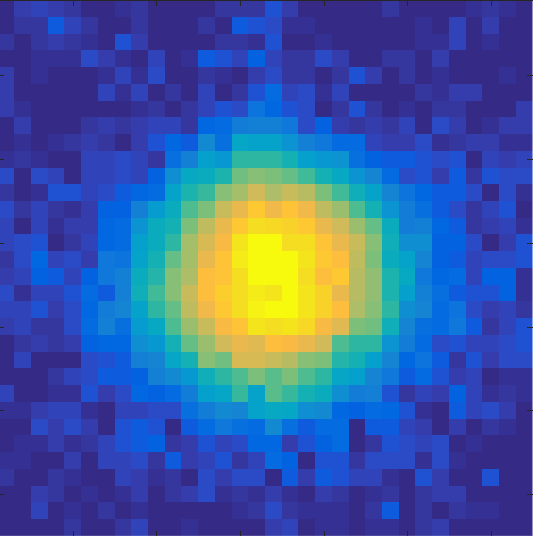
\includegraphics[width=0.19\linewidth]{img/chap4/CorrupPI_PS_clean}}
	\subfigure[PS inicial.]{\label{subfig:PI_ps_init}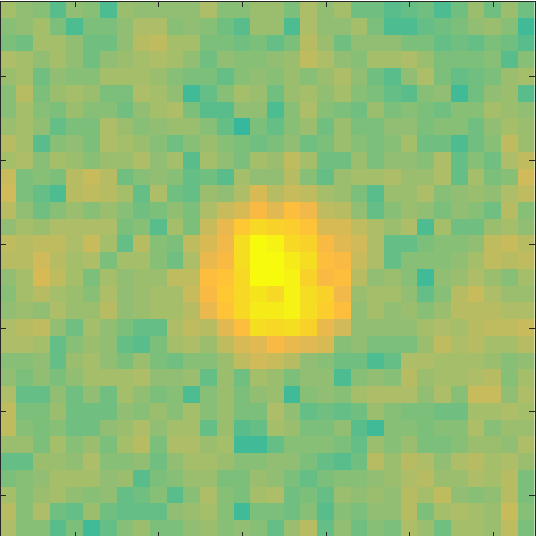
\includegraphics[width=0.19\linewidth]{img/chap4/CorrupPI_PS_init}}
	\subfigure[PS en la 2° iteración.]{\label{subfig:PI_ps_5iter}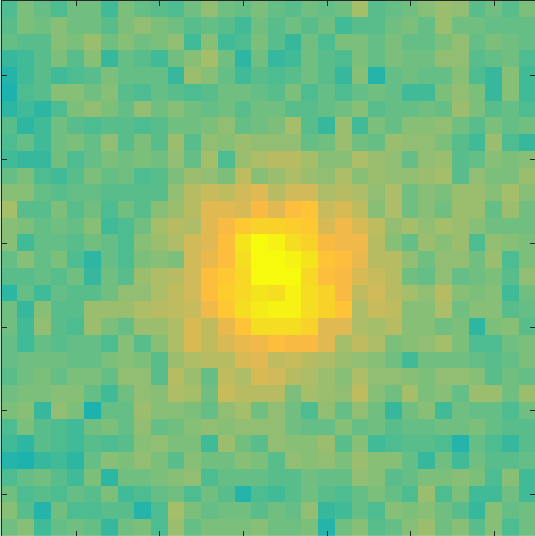
\includegraphics[width=0.19\linewidth]{img/chap4/CorrupPI_PS_5iter}}
	\subfigure[PS en la 4° iteración.]{\label{subfig:PI_ps_15iter}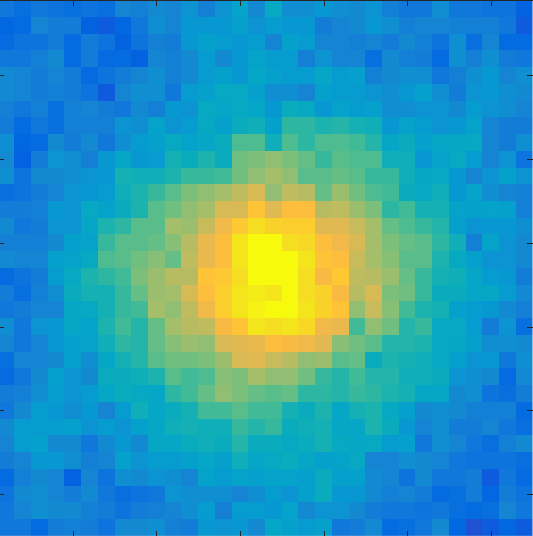
\includegraphics[width=0.19\linewidth]{img/chap4/CorrupPI_PS_15iter}}
	\subfigure[PS final $\hat{\zeta}(k)$.]{\label{subfig:PI_ps_30iter}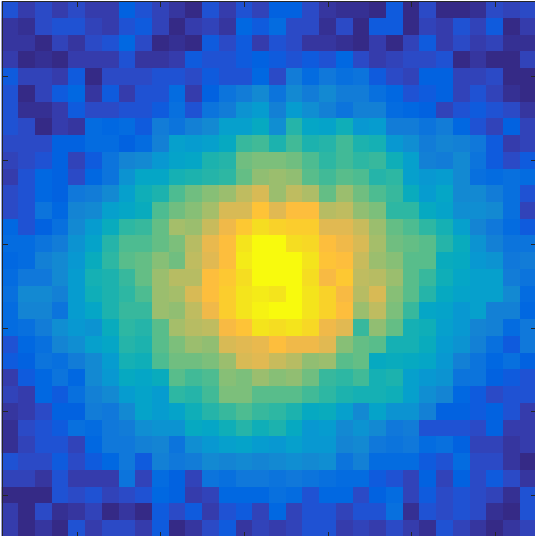
\includegraphics[width=0.19\linewidth]{img/chap4/CorrupPI_PS_30iter}}
	\caption[Espectros de potencia para una escala de corrupción aleatoria de $\pi$]{PS obtenidos en diferentes iteraciones del algoritmo para una corrupción aleatorio en un rango de $\pi$. (a) PS no corrupto, (b) PS inicial para el algoritmo, como la corrupción no es de $2\pi$, se observan características gaussianas en el haz; (c) PS recuperado en la 2° iteración del algoritmo, (d) PS en la 4° iteración del algoritmo, y (e) PS final calculado.}
	\label{fig:ps_pi}
\end{figure}

\begin{figure}[ht!]
	\centering
	\subfigure[Fase no corrupta.]{\label{subfig:PI_clean_phase}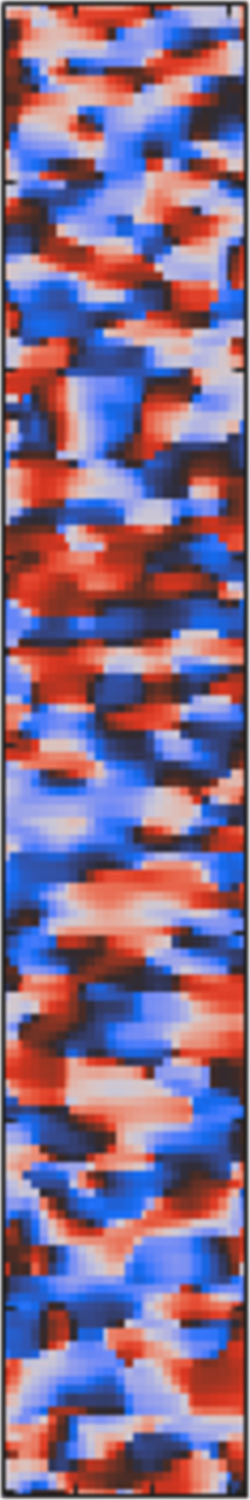
\includegraphics[width=2.5cm,height=8cm]{img/chap4/CorrupPI_phase_clean}}\hspace{1cm}
	\subfigure[Fase corrupta.]{\label{subfig:PI_corrupt_pase}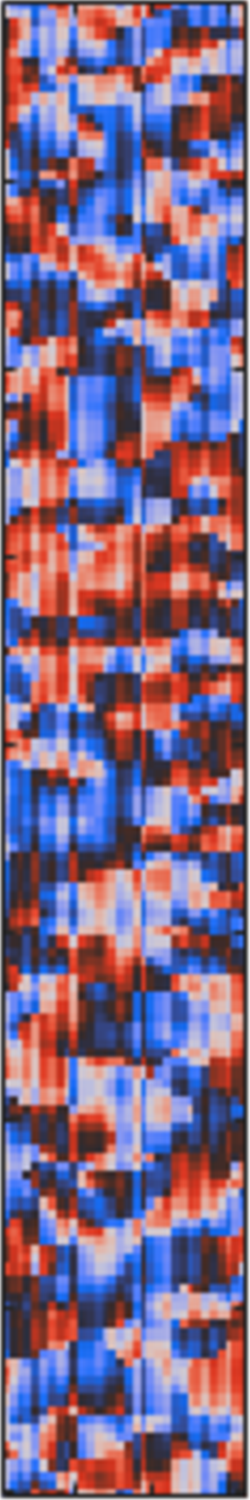
\includegraphics[width=2.5cm,height=8cm]{img/chap4/CorrupPI_phase_corru}}\hspace{1cm}
	\subfigure[Fase corregida.]{\label{subfig:PI_corrected_phase}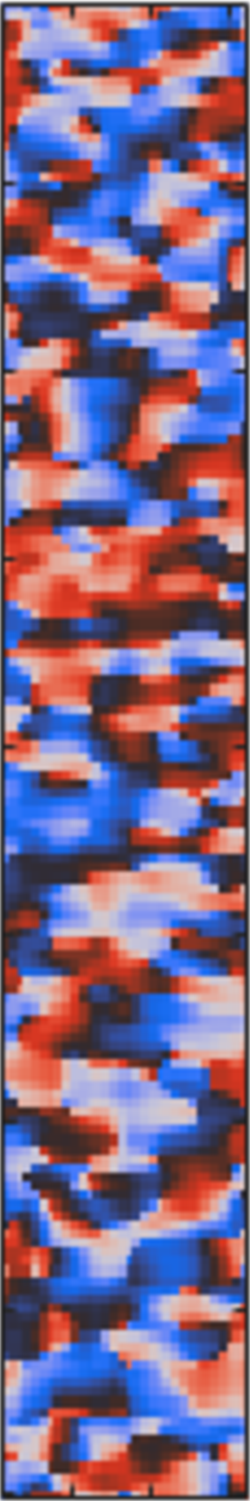
\includegraphics[width=2.5cm,height=8cm]{img/chap4/CorrupPI_phase_corrected}}
	\subfigure{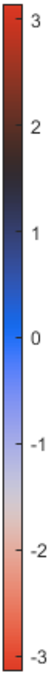
\includegraphics[width=0.6cm,height=8cm]{img/chap4/ColorbarCmapC3}}
	\caption[Fase recuperada para una escala de corrupción aleatoria de $\pi$]{Comparación de las fases sin corrupción (a) y con corrupción (b), respecto a la corregida (c) para una escala de corrupción de $\pi$. Nótese que pueden haber saltos de fase globales que no son perceptibles por el algoritmo.}
	\label{fig:phase_pi}
\end{figure}
%FUERON 40 ITERACIONES VOL SIZE 160X32X32
%PROBLEMA NO NECESARIAMENTE CONVEXO Y PODEMOS ESTAR ATASCADOS EN MINIMO LOCAL

Sin embargo, al incrementar la escala de los valores aleatorios para el \offset y la pendiente hasta un rango de $2\pi$, se notó que el algoritmo no lograba encontrar de manera óptima la solución. En las Figs.~\ref{fig:2pi_ps} y \ref{fig:2pi_phase} se presenta la comparación de los PS y las fases respectivamente cuando los valores aleatorios adquieren cualquier número entre $0$ y $2\pi$. En este caso, los PS muestran algunas diferencias significativas luego de la corrección, esto se aprecia al comparar el PS promedio final recuperado [Fig.~\ref{subfig:2pi_ps_30iter}] con respecto al PS promedio sin corrupción [Fig.~\ref{subfig:2pi_ps_clean}], de la misma manera, los PS en la segunda y cuarta iteración en las Figs.~\ref{subfig:2pi_ps_5iter} y \ref{subfig:2pi_ps_15iter} respectivamente exhiben que el algoritmo parece converger a un mínimo local. Al evaluar la función de mérito, su valor inicial era de $1140$, mientras que en la última iteración se logró un valor mínimo de $420$. El análisis de las fases antes [Fig.~\ref{subfig:2pi_phase_corrupt}] y después de la corrección [Fig.~\ref{subfig:2pi_phase_corrected}] manifestaron una fase corregida parcialmente, en donde todavía se evidencia elementos aleatorios asociados con la corrupción al compararlos con el tomograma limpio [Fig.~\ref{subfig:2pi_phase_clean}].

\begin{figure}[ht!]
	\centering
	\subfigure[PS no corrupto.]{\label{subfig:2pi_ps_clean}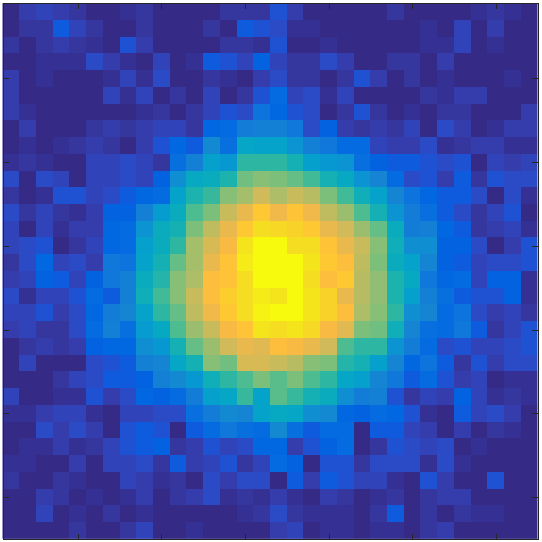
\includegraphics[width=0.19\linewidth]{img/chap4/Corrup2PI_ps_clean}}
	\subfigure[PS corrupto.]{\label{subfig:2pi_ps_init}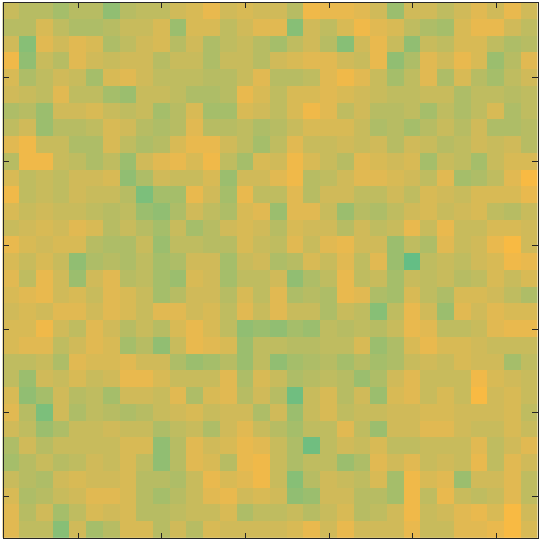
\includegraphics[width=0.19\linewidth]{img/chap4/Corrup2PI_ps_init}}
	\subfigure[PS en 2° iteración.]{\label{subfig:2pi_ps_5iter}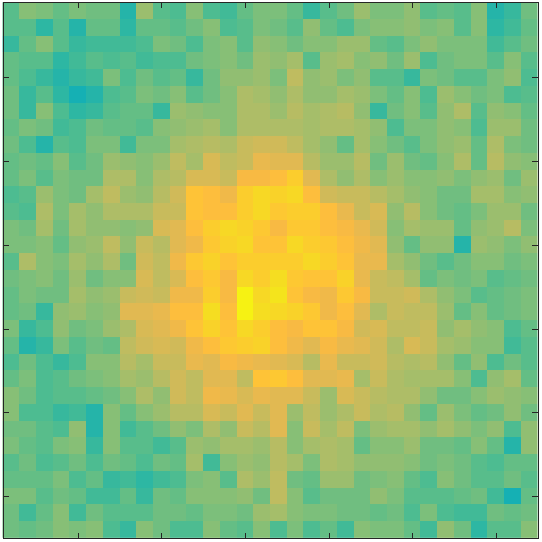
\includegraphics[width=0.19\linewidth]{img/chap4/Corrup2PI_ps_5iter}}
	\subfigure[PS en 4° iteración.]{\label{subfig:2pi_ps_15iter}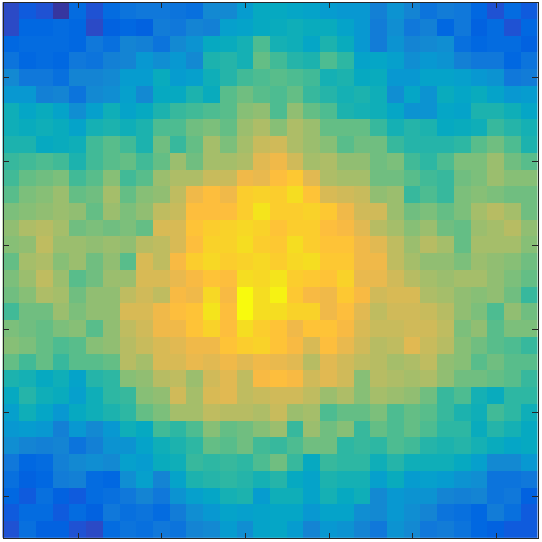
\includegraphics[width=0.19\linewidth]{img/chap4/Corrup2PI_ps_15iter}}
	\subfigure[PS final.]{\label{subfig:2pi_ps_30iter}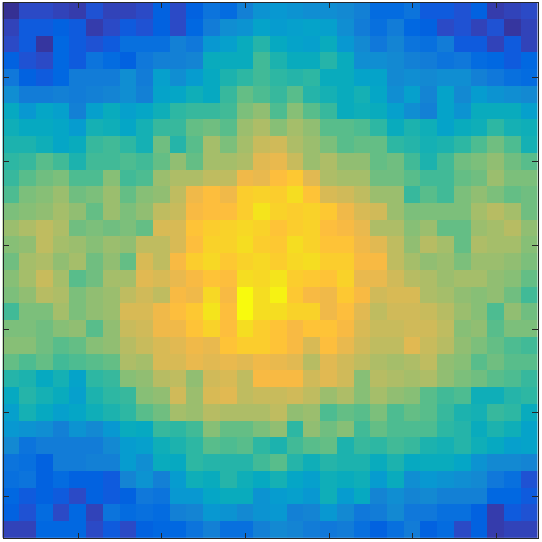
\includegraphics[width=0.19\linewidth]{img/chap4/Corrup2PI_ps_30iter}}
	\caption[Espectros de potencia para una escala de corrupción aleatoria de $2\pi$]{PS obtenidos en diferentes iteraciones del algoritmo para una corrupción aleatorio en un rango de $2\pi$. En este caso, no hay una buena estimación por parte del algoritmo.}
	\label{fig:2pi_ps}
\end{figure}

\begin{figure}[ht!]
	\centering
	\subfigure[Fase no corrupta.]{\label{subfig:2pi_phase_clean}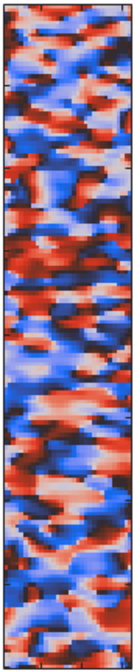
\includegraphics[width=2.5cm,height=8cm]{img/chap4/Corrup2PI_phase_clean}}\hspace*{1cm}
	\subfigure[Fase corrupta.]{\label{subfig:2pi_phase_corrupt}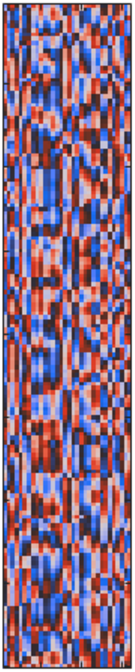
\includegraphics[width=2.5cm,height=8cm]{img/chap4/Corrup2PI_phase_corru}}\hspace*{1cm}
	\subfigure[Fase corregida.]{\label{subfig:2pi_phase_corrected}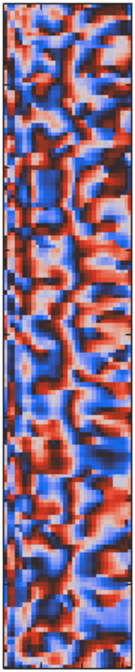
\includegraphics[width=2.5cm,height=8cm]{img/chap4/Corrup2PI_phase_corrected}}
	\subfigure{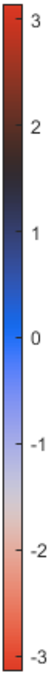
\includegraphics[width=0.6cm,height=8cm]{img/chap4/ColorbarCmapC3}}
	\caption[Fase recuperada para una escala de corrupción aleatoria de $2\pi$]{Comparación de las fases sin corrupción (a) y con corrupción (b), respecto a la corregida (c) para una escala de corrupción de $2\pi$. Se aprecia que la fase corregido aún posee elementos de corrupción.}
	\label{fig:2pi_phase}
\end{figure}



La evaluación de los distintos rangos de corrupción mostraron que el algoritmo funciona para valores del \offset y la pendiente inferiores a $1.3\pi$, en donde los resultados sugieren que el algoritmo converge a un mínimo local, la comparación de la función de mérito (FOM) obtenida contra la escala de los valores aleatorios de la pendiente y el \offset se presenta en la Fig.~\ref{fig:FOM_over_corrupt_scale}. Allí se observa que la solución final del algoritmo tiene una función de mérito superior a $100$ en donde su funcionamiento no es el esperado. Esta evaluación, permitió definir que un rango de valores de la función de mérito final entre $[0-60]$ producen una buena aproximación para el algoritmo, por el contrario, si la función de mérito final supera $\approx100$ sugiere que la solución está en un mínimo local, y por ende, no hay una buena reconstrucción del mapa de corrupción. Aun así, creemos que este resultado puede mejorarse si hay una semilla que le indique al algoritmo algunos de los valores de la pendiente y el \offset en la solución, puesto que como lo muestran las escalas bajas el algoritmo funciona ante corrupciones inferiores a $1.3\pi$. Para mejorar este problema, se sugiere entonces realizar un cálculo previo de una semilla y se plantea un nuevo método para evaluar cada línea A, buscando con esto extender el funcionamiento del algoritmo hasta aquellos rangos aleatorios cercanos a $2\pi$, valores que se esperan en los problemas experimentales.

\begin{figure}
	\centering
	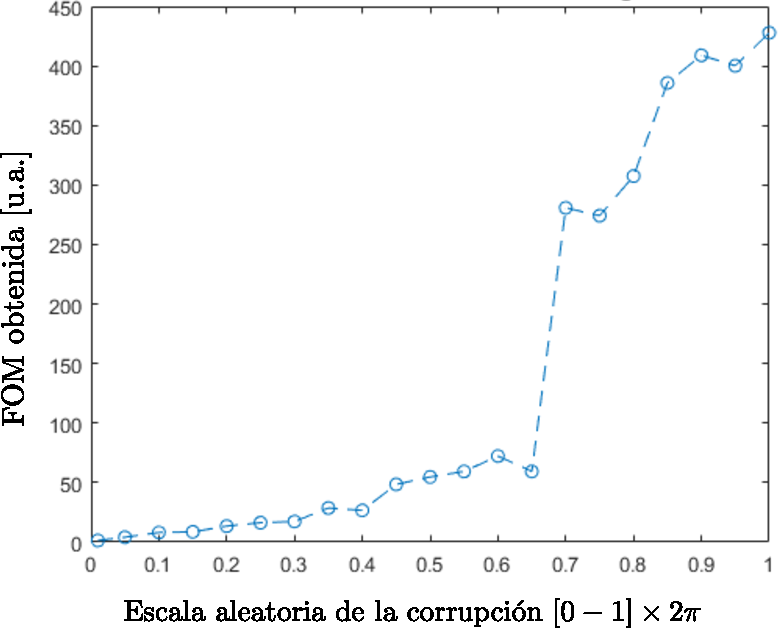
\includegraphics[width=0.4\linewidth]{img/chap4/FOM_over_corrupt_scale}
	\caption[Función de mérito final a partir de escala de corrupción.]{Función de mérito (FOM) final a partir de escala de corrupción, hasta un valor máximo de $0.65$ ($1.3\pi$) la FOM es menor a $100$, indicando la convergencia del algoritmo, sin embargo, no mejora la reconstrucción luego de este valor.}
	\label{fig:FOM_over_corrupt_scale}
\end{figure}

\subsection{Una semilla para el algoritmo}
\label{subsec:semilla}

%En vista de que el algoritmo de optimización para encontrar la pendiente y el \offset se ha propuesto un modelo de optimización que se soluciona mediante el cálculo iterativo de los valores reales. 

En vista de que el algoritmo propuesto se basa en una optimización para encontrar las pendientes y los \offset del tomograma corrupto, es susceptible a encontrar mínimos locales como solución, sin embargo, es posible indicar una semilla que sea el punto de partida para prevenir estos problemas. Se propone obtener un cálculo previo de las pendientes $\hat{\xi}_n$ y los \offset $\hat{\varphi}_n$ para dar una semilla, y que finalmente el algoritmo encuentre los parámetros optimizados. La propuesta está inspirada en el trabajo de Hong \etal \cite{Hong2012}, en donde calculan los parámetros de corrupción en un proceso de estabilización de dos pasos, primero una corrección mediante la correlación entre líneas A adyacentes, y posteriormente un ajuste de los saltos de fase residuales. La idea es emplear el primer paso del algoritmo de Hong \etal para realizar una estimación inicial de el \offset y la pendiente, y finalmente, se realizará el proceso de optimización mencionado anteriormente para recuperar el tomograma sin corrupción. 

Para calcular la semilla del algoritmo, asumiremos que dadas las características de las muestras analizadas por OFDI la fase entre dos líneas A adyacentes $F_n(z)$ y $F_{n+1}(z)$ no presenta variaciones significativas causadas por la muestra, sino que sus diferencias son ocasionadas principalmente por la falta de sincronía entre la fuente de barrido y el fotodetector. El proceso de estimación se realiza entonces en dos etapas, primero un cálculo del \offset y posteriormente la pendiente. Inicialmente, es necesario realizar la resta entre las fases de las dos líneas A $F_n(z)$ y $F_{n+1}(z)$ por medio del complejo conjugado $[\angle \{F_{n+1}(z)-F_n(z)\} = F_{n+1}(z)F_n^{\star}(z)]$, con $^\star$ la operación complejo conjugado y $\angle$ indica la parte compleja o fase, de modo que si la fase de la muestra entre las líneas A es aproximada, solamente se tendrá la influencia del \offset y la pendiente en $\angle \{F_{n+1}(z)-F_n(z)\}$.

El \offset corresponde entonces al valor medio de la diferencia de fase entre las líneas A para todas las profundidades, 

\begin{equation}
\hat{\varphi}_n = \frac{1}{N}\sum_{n=2}^{N}\angle\{ F_{n+1}(z)-F_n(z)\}.
\end{equation}

\noindent Para calcularlo, se realiza una normalización de la amplitud, reemplazando la proveniente de la muestra con una ventana gaussiana para evitar que los puntos con baja intensidad aporten fases aleatorias. Además, a cada \offset se le agregan los \textit{offsets} de las líneas A anteriores ya que éstos son acumulativos. Por último, se realiza un filtro paso alto para evitar errores por la acumulación de bajas frecuencias o pequeñas diferencias en la fase del objeto. 

En la estimación de la pendiente, se emplea el espectro de potencia de la resta compleja de las líneas A, tomando el módulo cuadrado de su transformada de Fourier $\lvert \mathscr{F}\{F_{n+1}(z)F_n^{\star}(z) \}\rvert^2$, luego se calcula la posición del pico en el espectro de potencia y se interpola su posición subpixel, para que aquellos valores inferiores a $2\pi$ sean considerados. Con esto, se ha calculado la diferencia de pendientes entre las líneas A, para tener el valor de la pendiente de cada línea es necesario sumarle a cada una la pendiente calculada para todas las anteriores, y realizar un filtro paso alto para evitar la acumulación de errores de baja frecuencia.

Para evaluar cada una de las líneas A que conforman el tomograma se propone comenzar con los puntos extremos $xy$ durante las primeras iteraciones e incrementar la cantidad de puntos evaluados gradualmente hasta que la totalidad de las líneas A sean calculadas. La razón para hacerlo en este orden, es que al aplicar las máscaras gaussianas antes de tomar las transformadas de Fourier en $XY$ aquellos puntos tienen bajos valores de amplitud, y es justamente en estos puntos, donde el algoritmo tiende a estar alejado de sus valores reales. Al evaluarlos múltiples veces en cada iteración, se estima primero sus parámetros de corrupción y como la información se añade gradualmente, estos puntos tenderán a aproximarse mejor a los parámetros reales.

Con este nuevo esquema de estimación de la semilla y evaluación de las líneas A se consiguió mejorar el algoritmo para emplearse en el caso de valores aleatorios de pendiente y \offset en un rango de $2\pi$, ya que como se esperaba, comenzar en una aproximación al resultado mejora notoriamente el desempeño del algoritmo. La comparación del PS recuperado y la fase corregida para variaciones del \offset y la pendiente en un rango de $0$ a $2\pi$ con la semilla del algoritmo se presentan en la Fig.~\ref{fig:ps_final} y la Fig.~\ref{fig:phase_final} respectivamente, para un volumen conformado por $N=64\times12$ líneas A y $M=160$ muestras de $z$.

En la Fig.~\ref{subfig:fin_ps_clean} se presenta el PS promedio inicial producido por el tomograma sin corrupción, su apariencia achatada se debe a que hay muchos más datos sobre uno de los ejes, la Fig.~\ref{subfig:fin_ps_init} es el PS promedio obtenido con el tomograma corrupto, la Fig.~\ref{subfig:fin_ps_seed} es el PS promedio luego de aplicar la semilla, nótese que ésta es muy similar a la corrupta, sin embargo, los valores de fase varían lo suficiente para dar un punto de partida para el algoritmo. La PS final luego de las 125 iteraciones con el nuevo procedimiento planteado se muestra en la Fig.~\ref{subfig:fin_ps_fin}, en donde se omitieron de manera gradual $\{8\times4, 6\times3, 4\times2, 2\times1, 0\times0\}$ líneas A, y en cada uno de esos saltos se valuaron intervalos de $\{6, 7, 9, 11, 13\}$ divisiones de $2\pi$. La función de mérito en este caso, tuvo un valor inicial de $1411$ y un valor final de $51$, el menor obtenido hasta ahora con el algoritmo. La comparación de los resultados, muestra que la reconstrucción presenta unas diferencias que se deben a que todavía no se ha terminado de obtener los mapas de corrupción exactos, a causa de que las evaluaciones discretas que realiza el algoritmo no permite tener valores que requieren alta precisión. Este problema se podría solucionar si se hace la evaluación de más puntos en el intervalo $j$.

Por último, en la Fig.~\ref{subfig:fin_phase_clean} se presenta la fase del tomograma sin corrupción, mientras que la Fig.~\ref{subfig:fin_phase_corrupt} corresponde a la fase corrupta, la Fig.~\ref{subfig:fin_phase_seed} es la fase con la semilla al iniciar el algoritmo y la Fig.~\ref{subfig:fin_phase_corrected} es la fase corregida con la pendiente y el \offset obtenidos, a esta fase se le aplicó un corrimiento de $0.7\pi$ global ya que un corrimiento en toda la fase no es detectable por el algoritmo. Los resultados de la fase muestran que mediante el procesamiento del volumen, la aplicación de la corrupción inversa encontrada mejora notoriamente la fase inicial del tomograma, fuertemente alterada. La fase ilustra la eliminación de la corrupción casi en su totalidad, excepto en algunas pequeñas regiones en donde la estimación no arrojó valores completamente acertados, ya que finalmente, estamos realizando una aproximación al mapa de corrupción. Estos resultados muestran que el algoritmo es capaz de recuperar cualquier corrupción con pendientes aleatorias y \textit{offsets} aleatorios en un rango de $0$ a $2\pi$, se espera que este rango sea suficiente para corregir la falta de sincronía entre la fuente y el detector, en donde un desfase superior a un ciclo indicaría que la pendiente es mayor a $2\pi$. 

\begin{figure}[ht!]
	\centering
	\subfigure[PS no corrupto.]{\label{subfig:fin_ps_clean}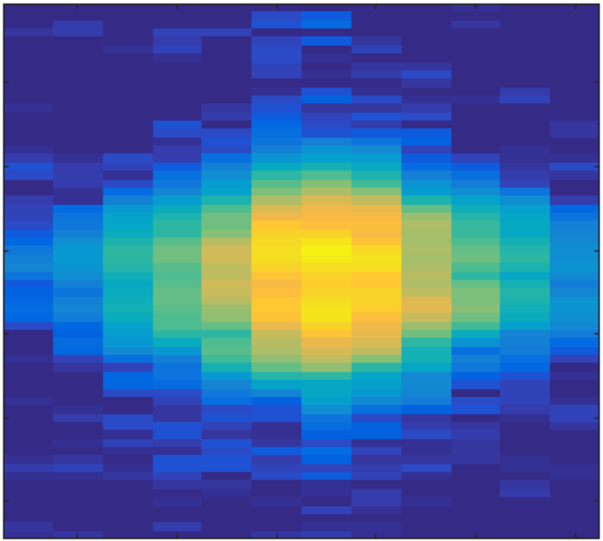
\includegraphics[width=0.24\linewidth]{img/chap4/Final_PS_clean}}
	\subfigure[PS corrupto.]{\label{subfig:fin_ps_init}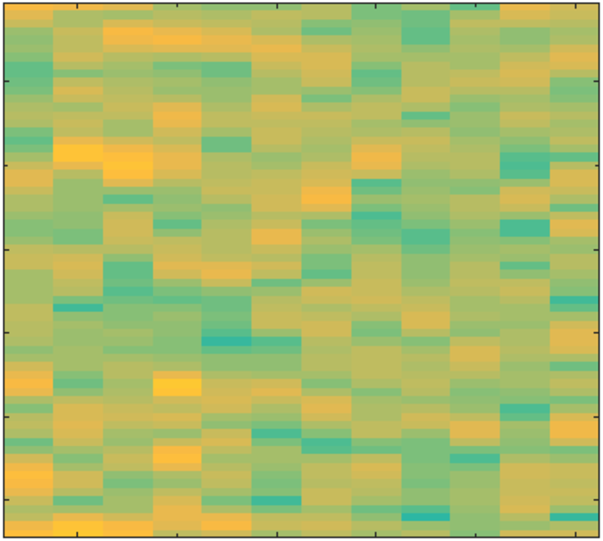
\includegraphics[width=0.24\linewidth]{img/chap4/Final_PS_init}}
	\subfigure[PS semilla.]{\label{subfig:fin_ps_seed}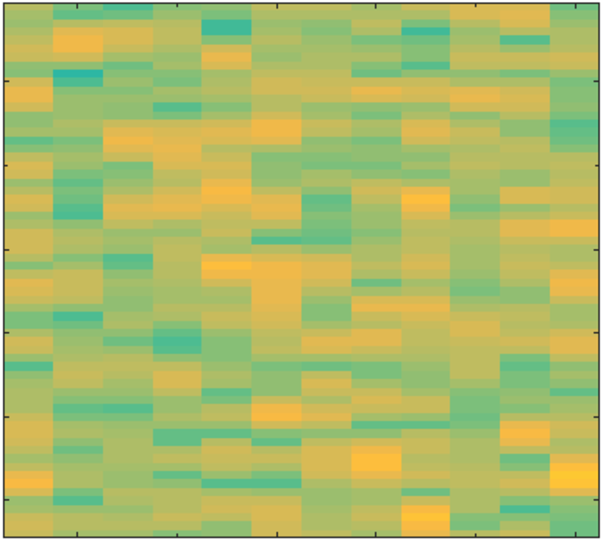
\includegraphics[width=0.24\linewidth]{img/chap4/Final_PS_seed}}
	\subfigure[PS final.]{\label{subfig:fin_ps_fin}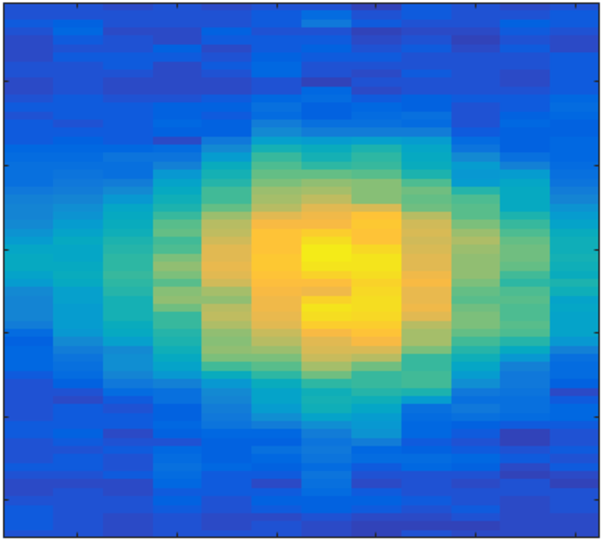
\includegraphics[width=0.24\linewidth]{img/chap4/Final_PS_calc}}
	\caption[Espectro de potencia obtenido en diferentes iteraciones del algoritmo de optimización]{PS obtenidos en diferentes iteraciones del algoritmo para una corrupción aleatorio en un rango de $2\pi$ con las mejoras propuestas. Se observa que hay una mejora notable en la reconstrucción que realiza el algoritmo, esto se refleja en la disminución del mínimo en la función de mérito.}
	\label{fig:ps_final}
\end{figure}


\begin{figure}[ht!]
	\centering
	\subfigure[Fase no corrupta.]{\label{subfig:fin_phase_clean}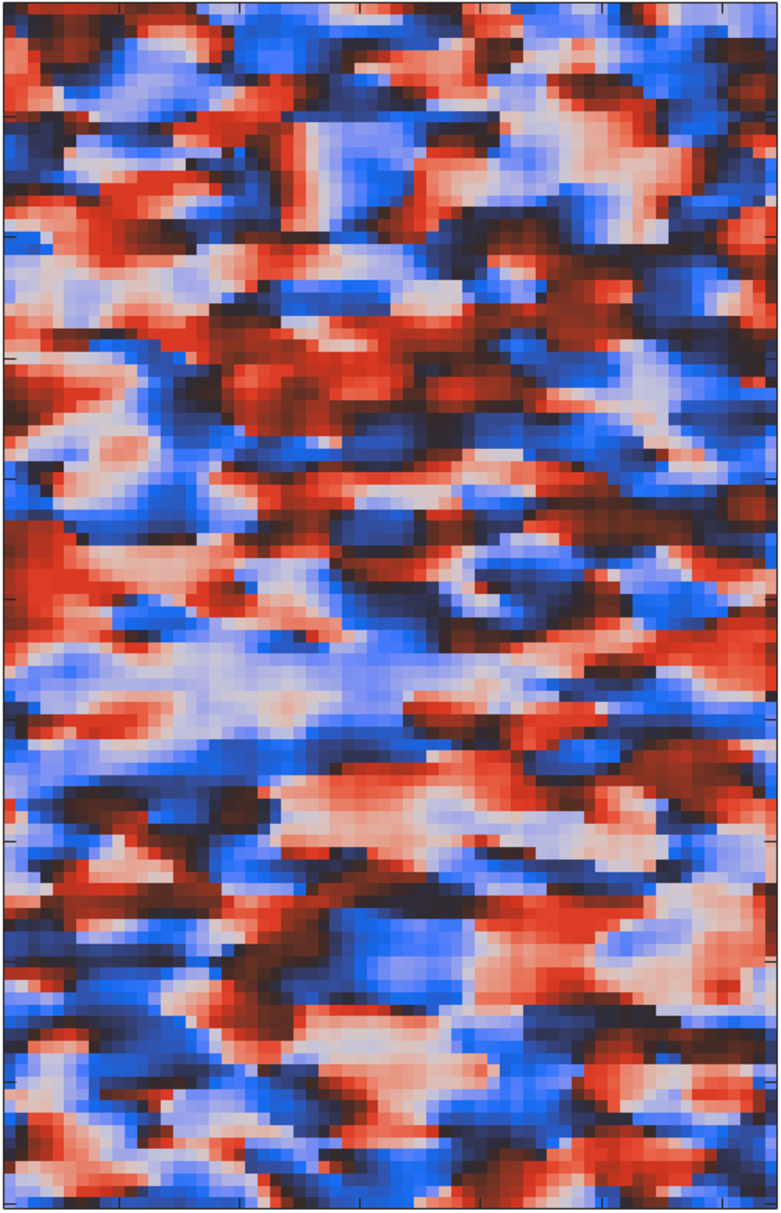
\includegraphics[width=0.23\linewidth]{img/chap4/Final_phase_clean}}
	\subfigure[Fase corrupta.]{\label{subfig:fin_phase_corrupt}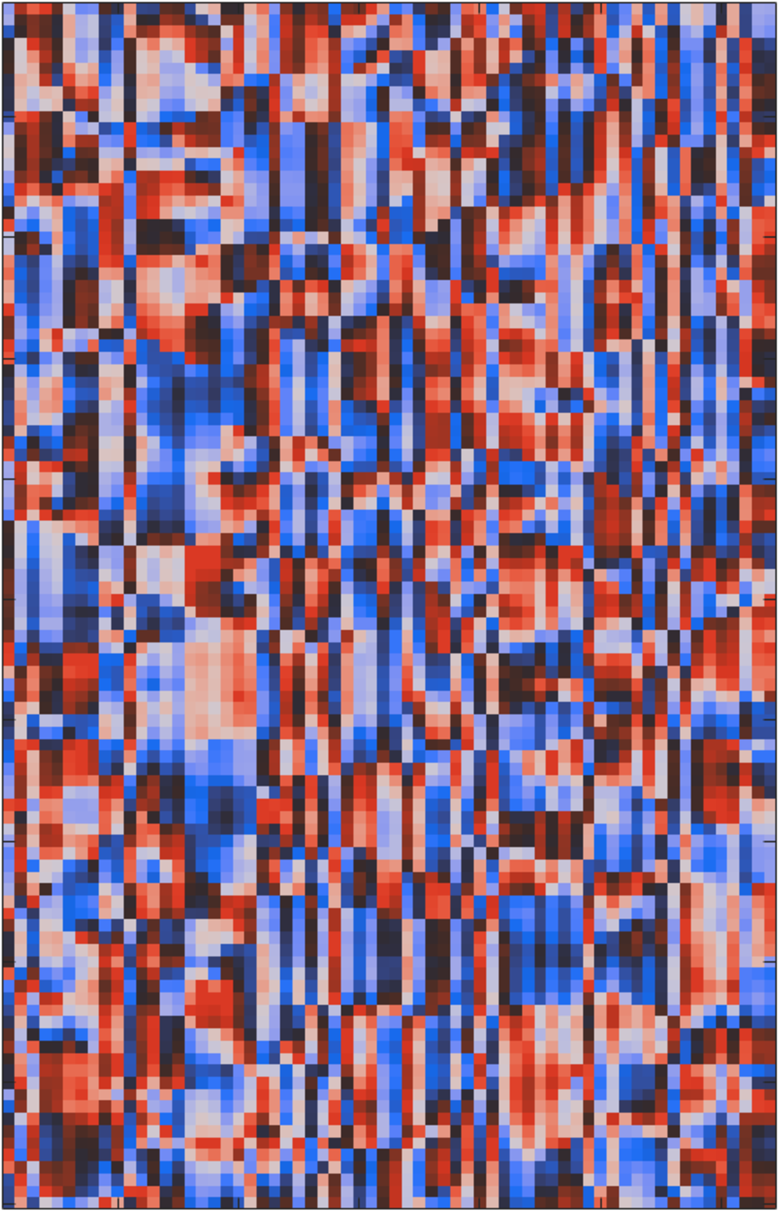
\includegraphics[width=0.23\linewidth]{img/chap4/Final_phase_corrupt}}
	\subfigure[Fase semilla.]{\label{subfig:fin_phase_seed}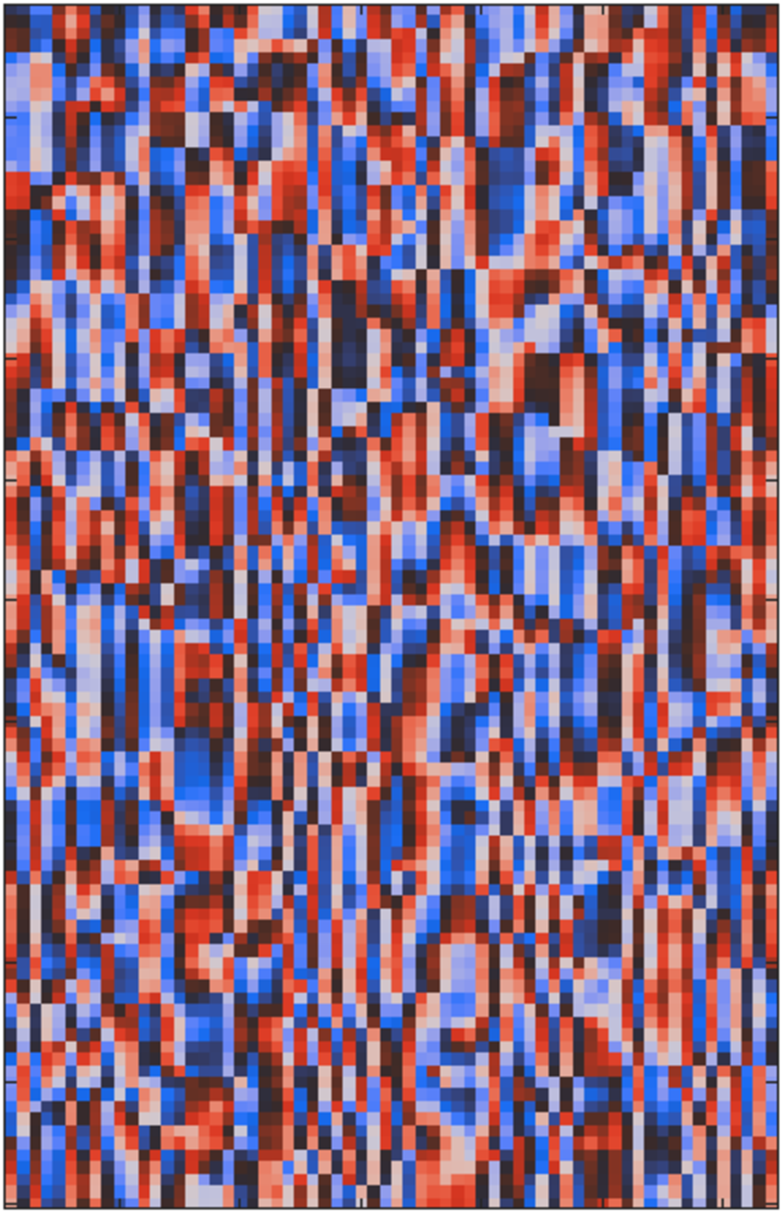
\includegraphics[width=0.23\linewidth]{img/chap4/Final_phase_at_seed}}
	\subfigure[Fase corregida.]{\label{subfig:fin_phase_corrected}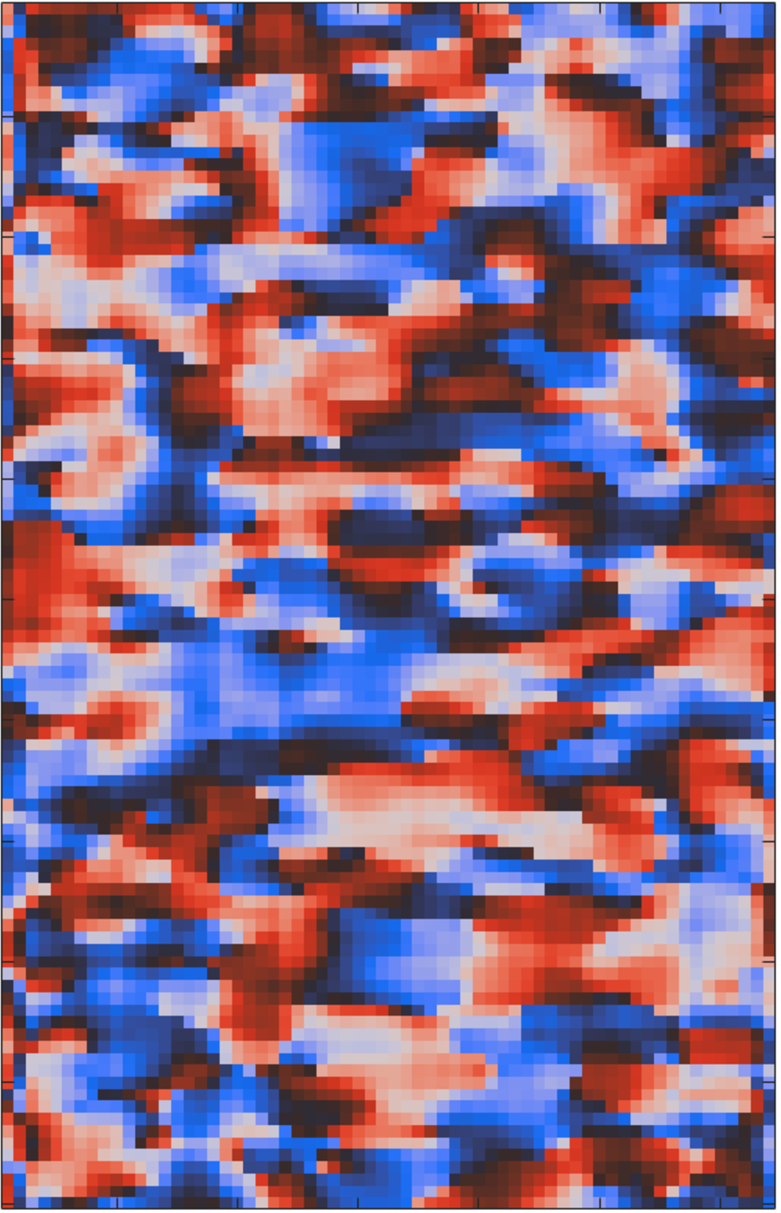
\includegraphics[width=0.23\linewidth]{img/chap4/Final_phase_corrected}}
	\subfigure{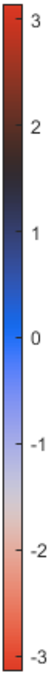
\includegraphics[width=0.0275\linewidth]{img/chap4/ColorbarCmapC3}}
	\caption[Comparación de la fase recuperada con la optimización]{Comparación de las fases sin corrupción (a) y con corrupción (b), en la semilla del algoritmo y (d) corregida, para valores aleatorios de $2\pi$. A la fase corregida se le aplicó un corrimiento de fase global que no es detectable. La fase corregida en este caso, sigue un comportamiento muy similar a la fase sin corrupción.}
	\label{fig:phase_final}
\end{figure}

%Una de las modalidades de imagen en OCT, se basa en la captura del patrón de interferencia que se produce entre la porción de luz retroreflejada por la muestra con el haz de referencia mediante una fuente de barrido. A esta aplicación se le denomina OCT con fuente de barrido (SSOCT: \textit{swept-source optical coherence tomography}), en este caso, se produce la interferencia con secciones angostas del espectro de la fuente, mientras se realiza un barrido por todo el espectro. El patrón de interferencia se captura finalmente con un fotodetector, que almacena la reflectividad de la muestra como una función del número de onda $k$ %\cite{Drexler2015}. 

\section{Resultados experimentales preliminares}
\label{sec:resultados_experimentales_ofdi}

Con respecto al algoritmo para recuperar el mapa de corrupción a partir de la optimización de la fase, se tienen resultados experimentales preliminares, que reflejan el funcionamiento del algoritmo con datos provenientes de un sistema de OFDI. No obstante, los resultados presentados en esta sección se encuentran todavía en procesamiento, y son la ilustración de los problemas que esperamos poder mejorar antes de aplicar el procedimiento propuesto en un tomograma entero. Para las pruebas experimentales, se utilizaron los datos provenientes del cerebro de ratón obtenidos con OCT luego del procedimiento de \textit{blanqueado} y escaneo mediante OFDI descrito en detalle en la Sección~\ref{sec:oct_tractography}. Otro problema que tienen los datos del escaneo del cerebro con OFDI, además del ruido por \speckle ya mencionado, es que la información de fase se pierde por la falta de sincronía, que genera corrupciones en la fase. En este caso, la fase es particularmente interesante, ya que como lo ha demostrado Chen \etal \cite{Chen2009}, OCT tiene el potencial de develar actividad cerebral. Este procedimiento podría realizarse mediante mediciones de flujo, que como se ha mencionado dependen de la fase que presenta problemas ligados a la instrumentación. En este caso, se utilizó un recorte de las sinapsis del cerebro de $300\times64\times20$, en donde se ha tomado parte de la profundidad del cerebro de ratón que se encuentra por fuera de la región focal, y se han considerado algunos escaneos B que contienen información relevante de las sinapsis.

Para el cálculo se empleó el procedimiento descrito en la Sección~\ref{subsec:semilla}, con los parámetros allí especificados. Pese a que no conocemos el tomograma sin corrupción, más que interesados en el valor inicial y final de función de mérito, nos centramos en los cambios que se producen en ésta, en donde se partió de un valor de $1913$ y se obtuvo un mínimo con un valor de $750$. Los resultados obtenidos para el PS promedio tomando las respectivas transformadas de Fourier se presentan en la Fig.~\ref{fig:exp_ps}. La Fig.~\ref{subfig:exp_ps_clean} presenta la PS no corrupta propuesta, como se sugirió anteriormente, se ha tomado una función gaussiana. La Fig.~\ref{subfig:exp_ps_init} corresponde al espectro de potencia inicial del tomograma, en donde se observa la presencia de frecuencias distribuidas casi aleatoriamente. En la Fig.~\ref{subfig:exp_ps_seed} se expone la PS luego de realizar el proceso de obtención de semilla sugerido, nótese que en este caso la información del haz gaussiano empieza a aparecer, y en este punto comienza el algoritmo de optimización de fase. Posteriormente al procedimiento planteado, con un tiempo de procesamiento total de $6.3$ horas, se obtuvo el PS \textit{enfocado} que se presenta en la Fig.~\ref{subfig:exp_ps_fin}, en donde se aprecia la mejora sustancial que ha tenido el espectro de potencia sobre el plano $XY$. La presencia de algunas frecuencias altas se debe a que tanto la muestra como el ruido producen frecuencias que no se consideran en el espectro propuesto $\zeta^\dagger(k)$, y por ende, éstas no son calculadas por el algoritmo. Ésta figura sugiere que la reconstrucción del algoritmo fue satisfactoria en la mayor parte de las líneas A, sin embargo, dada la presencia de algunas altas frecuencias, habrán líneas A que todavía poseen algún grado de corrupción. Una posible explicación a esto, es que el algoritmo finalmente aproxima la solución para una pendiente inferior a $2\pi$, y probablemente el sistema de medida pudo sufrir desfases mayores a esta magnitud. Este problema podría solucionarse incrementando el rango de valores evaluados en la pendiente.

\begin{figure}[ht!]
	\centering
	\subfigure[PS no corrupto.]{\label{subfig:exp_ps_clean}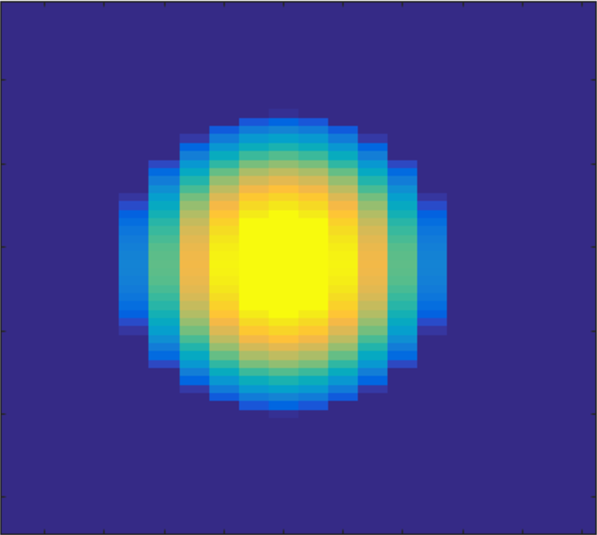
\includegraphics[width=0.24\linewidth]{img/chap4/exp_psf_clean}}
	\subfigure[PS corrupto.]{\label{subfig:exp_ps_init}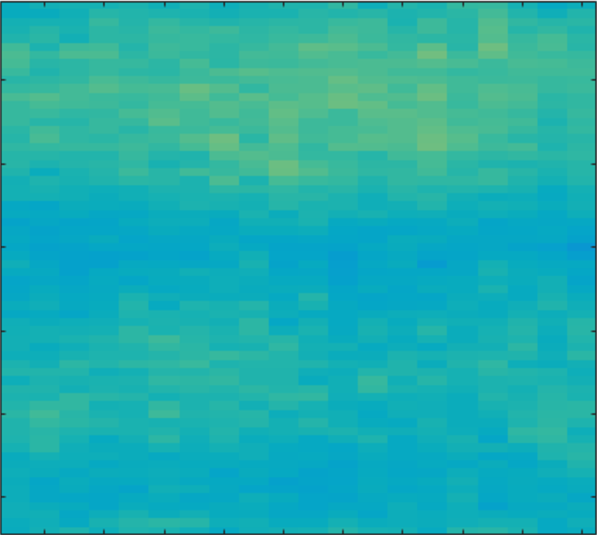
\includegraphics[width=0.24\linewidth]{img/chap4/exp_psf_init}}
	\subfigure[PS semilla.]{\label{subfig:exp_ps_seed}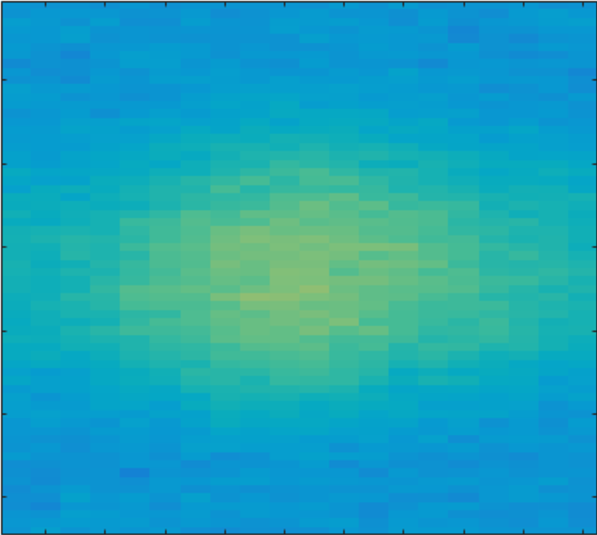
\includegraphics[width=0.24\linewidth]{img/chap4/exp_psf_at_seed}}
	\subfigure[PS final.]{\label{subfig:exp_ps_fin}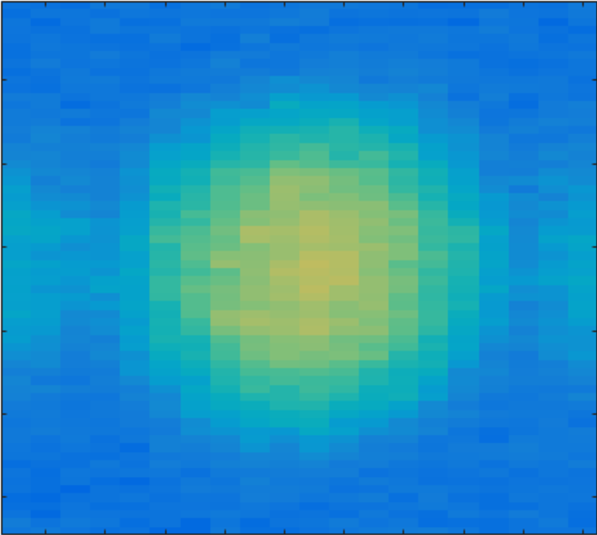
\includegraphics[width=0.24\linewidth]{img/chap4/exp_psf_final}}
	\caption[Espectros de potencia con datos experimentales]{Comparación de espectros de potencia obtenidos empleando el algoritmo de optimización de fase con datos experimentales, se tomaron los datos provenientes del cerebro de ratón. Se observa la mejora significativa en el PS producido por los datos corregidos con respecto a los iniciales.}
	\label{fig:exp_ps}
\end{figure}

Finalmente, la comparación de las fases para un escaneo B del subvolumen se presenta en la Fig.~\ref{fig:exp_phase}, en donde la Fig.~\ref{subfig:exp_phase_clean} presenta la intensidad del escaneo B comparado, la Fig.~\ref{subfig:exp_phase_corrupt} es la fase inicial del escaneo B, en donde claramente se aprecia la corrupción de fase; la Fig.~\ref{subfig:exp_phase_seed} corresponde a la fase corregida en la semilla del algoritmo, y finalmente, la Fig.~\ref{subfig:exp_phase_corrected} presenta la fase de emplear el algoritmo con los parámetros descritos. La comparación de la fase permite ver cómo en la semilla del algoritmo, ya hay una mejora significativa con respecto al tomograma corrupto, no obstante, se observa la presencia de algunos elementos de corrupción remanentes que posteriormente son corregidos en su gran mayoría por la optimización planteada. 

Nótese que en la región focal de la imagen, hacia la parte central, la fase presenta un comportamiento \textit{suave}, como el observado en las simulaciones, mientras que las regiones por fuera de la zona focal continúan teniendo problemas de corrupción. Estos errores que se presentan en la fase corregida, pueden ser ocasionados porque no se ha considerado que los haces gaussianos por fuera de la región focal tienen un desenfoque intrínseco, relacionado con las propiedades de este tipo de haz. Su consideración probablemente mejore notoriamente el resultado obtenido. Con respecto a la región focal de la imagen, en la banda central, es la misma región con la cual se realizó el filtrado del ruido por \speckle y es donde mejor se tiene una fase bien comportada que muestra un buen resultado inicial por parte de la optimización. Se espera poder mejorar este resultado empleando más líneas A del volumen, así como la consideración de más características relacionadas con el sistema experimental y que no se han realizado en estas pruebas preliminares, sin embargo, esto se plantea como trabajo futuro relacionado con la estabilización de la fase.


\begin{figure}[ht!]
	\centering
	\subfigure[Intensidad.]{\label{subfig:exp_phase_clean}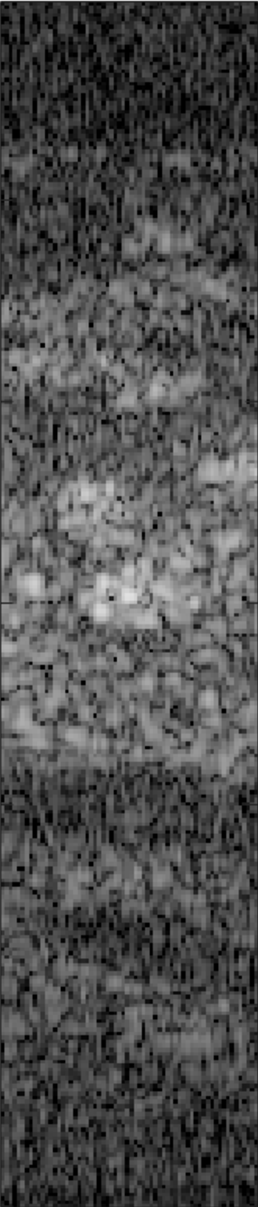
\includegraphics[width=0.23\linewidth]{img/chap4/exp_intensity}}
	\subfigure[Fase corrupta.]{\label{subfig:exp_phase_corrupt}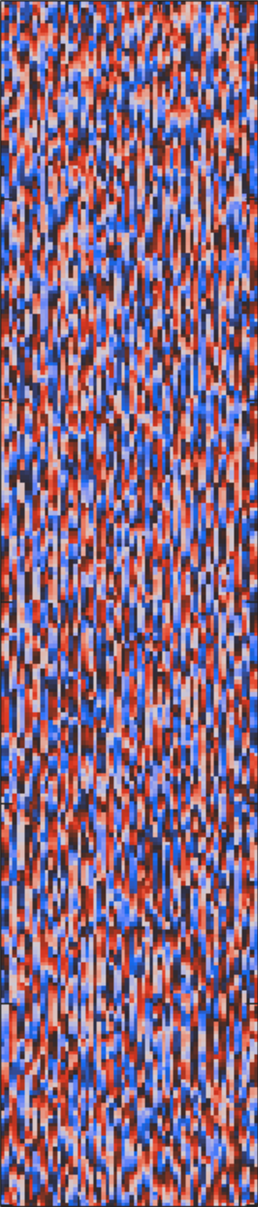
\includegraphics[width=0.23\linewidth]{img/chap4/exp_phase_corrupt}}
	\subfigure[Fase en la semilla.]{\label{subfig:exp_phase_seed}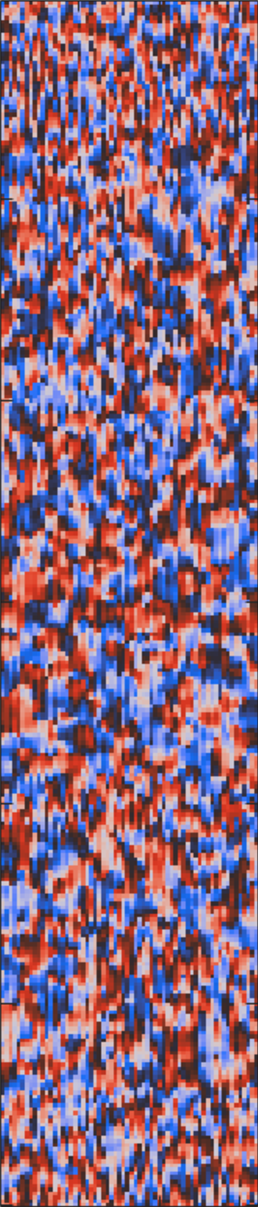
\includegraphics[width=0.23\linewidth]{img/chap4/exp_phase_at_seed}}
	\subfigure[Fase corregida.]{\label{subfig:exp_phase_corrected}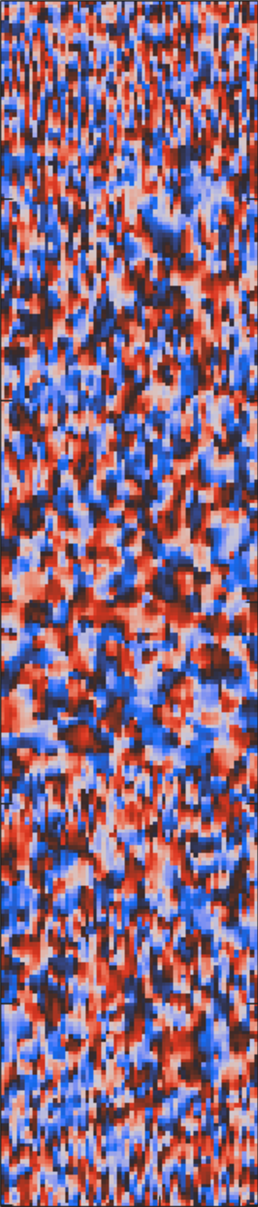
\includegraphics[width=0.23\linewidth]{img/chap4/exp_phase_corrected}}
	%\subfigure{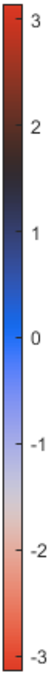
\includegraphics[width=0.0838\linewidth]{img/chap4/ColorbarCmapC3}}
	\caption[Comparación de la fase recuperada con la optimización en datos experimentales]{Comparación de las fases obtenidas con los datos experimentales provenientes del cerebro de ratón. La corrupción de la fase inicial se corrige en gran parte al evaluar la semilla, sin embargo, con el algoritmo de optimización se termina de mejorar este resultado. Las imágenes muestran que la región focal es donde la reconstrucción tiene un mejor comportamiento, esto puede estar relacionado con la región focal del haz.}
	\label{fig:exp_phase}
\end{figure}

\bibliographystyle{unsrt}
\bibliography{ref/Ref_chap_4}